% Import du style (obligatoire)
% Un template bilingue pour la production des mémoires et thèses dans le département de Mathématiques-Informatique.
% Ce template est conforme aux recommandations de l'école doctorale
%
% Ce fichier est le fichier de style principal. Vous y trouverez toutes les définitions des commandes personnalisées
%
% @author Zekeng Ndadji Milliam Maxime

\documentclass[12pt, a4paper, openany, oneside]{memoir}
\usepackage[T1]{fontenc}
\usepackage[utf8]{inputenc}
\usepackage{pifont}
\usepackage{pslatex}
%\usepackage{charter}
%\usepackage{mathptmx}
\usepackage{yfonts}
\usepackage[mathscr]{euscript}
\usepackage{latexsym}
\usepackage{stmaryrd}
\usepackage{amssymb}
\usepackage{amsmath}
\usepackage{graphicx}
\usepackage{pst-all}
\usepackage{verbatim} 
\usepackage{fancyvrb}%Pour utiliser l'environnement "Verbatim"
\usepackage{mathrsfs}
\usepackage{vmargin}
\usepackage{titletoc}
\usepackage{bbding}
\usepackage{wasysym}
%\usepackage{eufrak}
\usepackage{ifthen}
\usepackage[final]{pdfpages}
%\usepackage{natbib}
%\usepackage[natbibapa]{apacite}
\usepackage{morewrites}
\usepackage{tocbibind}
\usepackage{multicol}
% \usepackage{pdfpages}
% \usepackage{natbib}
% \usepackage[backend=biber,style=alphabetic,sorting=ynt]{biblatex}
% \addbibresource{My-thesis/bibliographiy.bib}
% \input{My-thes}
 
%\setpapersize{A4}
\DeclareMathAlphabet{\mathpzc}{OT1}{pzc}{m}{it}

\newcommand{\mathbox}[1]{\mbox{{\small \mbox{$ #1 $}}}}
\newcommand{\sta}[3]{\mathbox{#1 \stackrel{#2}{\longrightarrow} #3}}
\newcommand\QEDBox
{{\leavevmode\unskip\nobreak\hfil\penalty50\hskip.75cm%
    \hbox{} \nobreak\hfil $\Box$ \parfillskip=0pt
    \finalhyphendemerits=0
    \par
}}
\def\qed{\QEDBox}
\makeatletter
% *************** Définitions de quelques couleurs ***************
\usepackage{color}
\usepackage{colortbl}

\definecolor{greenyellow}   {cmyk}{0.15, 0   , 0.69, 0   }
\definecolor{yellow}        {cmyk}{0   , 0   , 1   , 0   }
\definecolor{goldenrod}     {cmyk}{0   , 0.10, 0.84, 0   }
\definecolor{dandelion}     {cmyk}{0   , 0.29, 0.84, 0   }
\definecolor{apricot}       {cmyk}{0   , 0.32, 0.52, 0   }
\definecolor{peach}         {cmyk}{0   , 0.50, 0.70, 0   }
\definecolor{melon}         {cmyk}{0   , 0.46, 0.50, 0   }
\definecolor{yelloworange}  {cmyk}{0   , 0.42, 1   , 0   }
\definecolor{orange}        {cmyk}{0   , 0.61, 0.87, 0   }
\definecolor{burntorange}   {cmyk}{0   , 0.51, 1   , 0   }
\definecolor{bittersweet}   {cmyk}{0   , 0.75, 1   , 0.24}
\definecolor{redorange}     {cmyk}{0   , 0.77, 0.87, 0   }
\definecolor{mahogany}      {cmyk}{0   , 0.85, 0.87, 0.35}
\definecolor{maroon}        {cmyk}{0   , 0.87, 0.68, 0.32}
\definecolor{brickred}      {cmyk}{0   , 0.89, 0.94, 0.28}
\definecolor{red}           {cmyk}{0   , 1   , 1   , 0   }
\definecolor{orangered}     {cmyk}{0   , 1   , 0.50, 0   }
\definecolor{rubinered}     {cmyk}{0   , 1   , 0.13, 0   }
\definecolor{wildstrawberry}{cmyk}{0   , 0.96, 0.39, 0   }
\definecolor{salmon}        {cmyk}{0   , 0.53, 0.38, 0   }
\definecolor{carnationpink} {cmyk}{0   , 0.63, 0   , 0   }
\definecolor{magenta}       {cmyk}{0   , 1   , 0   , 0   }
\definecolor{violetred}     {cmyk}{0   , 0.81, 0   , 0   }
\definecolor{rhodamine}     {cmyk}{0   , 0.82, 0   , 0   }
\definecolor{mulberry}      {cmyk}{0.34, 0.90, 0   , 0.02}
\definecolor{redviolet}     {cmyk}{0.07, 0.90, 0   , 0.34}
\definecolor{fuchsia}       {cmyk}{0.47, 0.91, 0   , 0.08}
\definecolor{lavender}      {cmyk}{0   , 0.48, 0   , 0   }
\definecolor{thistle}       {cmyk}{0.12, 0.59, 0   , 0   }
\definecolor{orchid}        {cmyk}{0.32, 0.64, 0   , 0   }
\definecolor{darkorchid}    {cmyk}{0.40, 0.80, 0.20, 0   }
\definecolor{purple}        {cmyk}{0.45, 0.86, 0   , 0   }
\definecolor{plum}          {cmyk}{0.50, 1   , 0   , 0   }
\definecolor{violet}        {cmyk}{0.79, 0.88, 0   , 0   }
\definecolor{royalpurple}   {cmyk}{0.75, 0.90, 0   , 0   }
\definecolor{blueviolet}    {cmyk}{0.86, 0.91, 0   , 0.04}
\definecolor{periwinkle}    {cmyk}{0.57, 0.55, 0   , 0   }
\definecolor{cadetblue}     {cmyk}{0.62, 0.57, 0.23, 0   }
\definecolor{cornflowerblue}{cmyk}{0.65, 0.13, 0   , 0   }
\definecolor{midnightblue}  {cmyk}{0.98, 0.13, 0   , 0.43}
\definecolor{navyblue}      {cmyk}{0.94, 0.54, 0   , 0   }
\definecolor{royalblue}     {cmyk}{1   , 0.50, 0   , 0   }
\definecolor{blue}          {cmyk}{1   , 1   , 0   , 0   }
\definecolor{cerulean}      {cmyk}{0.94, 0.11, 0   , 0   }
\definecolor{cyan}          {cmyk}{1   , 0   , 0   , 0   }
\definecolor{processblue}   {cmyk}{0.96, 0   , 0   , 0   }
\definecolor{skyblue}       {cmyk}{0.62, 0   , 0.12, 0   }
\definecolor{turquoise}     {cmyk}{0.85, 0   , 0.20, 0   }
\definecolor{tealblue}      {cmyk}{0.86, 0   , 0.34, 0.02}
\definecolor{aquamarine}    {cmyk}{0.82, 0   , 0.30, 0   }
\definecolor{bluegreen}     {cmyk}{0.85, 0   , 0.33, 0   }
\definecolor{emerald}       {cmyk}{1   , 0   , 0.50, 0   }
\definecolor{junglegreen}   {cmyk}{0.99, 0   , 0.52, 0   }
\definecolor{seagreen}      {cmyk}{0.69, 0   , 0.50, 0   }
\definecolor{green}         {cmyk}{1   , 0   , 1   , 0   }
\definecolor{forestgreen}   {cmyk}{0.91, 0   , 0.88, 0.12}
\definecolor{pinegreen}     {cmyk}{0.92, 0   , 0.59, 0.25}
\definecolor{limegreen}     {cmyk}{0.50, 0   , 1   , 0   }
\definecolor{yellowgreen}   {cmyk}{0.44, 0   , 0.74, 0   }
\definecolor{springgreen}   {cmyk}{0.26, 0   , 0.76, 0   }
\definecolor{olivegreen}    {cmyk}{0.64, 0   , 0.95, 0.40}
\definecolor{rawsienna}     {cmyk}{0   , 0.72, 1   , 0.45}
\definecolor{sepia}         {cmyk}{0   , 0.83, 1   , 0.70}
\definecolor{brown}         {cmyk}{0   , 0.81, 1   , 0.60}
\definecolor{tan}           {cmyk}{0.14, 0.42, 0.56, 0   }
\definecolor{gray}          {cmyk}{0   , 0   , 0   , 0.50}
\definecolor{black}         {cmyk}{0   , 0   , 0   , 1   }
\definecolor{white}         {cmyk}{0   , 0   , 0   , 0   } 

\usepackage{memhfixc}


% *************** Style de chapitre et de section ***************
\newcommand{\myPrintChapterLabel}[1]{
	\ifthenelse{\equal{#1}{A}}
		{\myAppendixLabel} 
		{\ifthenelse{\equal{#1}{B}}
			{\myAppendixLabel} 
			{\ifthenelse{\equal{#1}{C}}
				{\myAppendixLabel} 
				{\ifthenelse{\equal{#1}{D}}
					{\myAppendixLabel} 
					{\ifthenelse{\equal{#1}{E}}
						{\myAppendixLabel} 
						{\ifthenelse{\equal{#1}{F}}
							{\myAppendixLabel} 
							{\ifthenelse{\equal{#1}{G}}
								{\myAppendixLabel} 
								{\myChapterLabel}}}}}}} 
}

\newcommand{\StyleFolder}{../Template-Style}
\newcommand{\ChapterStylesFolder}{\StyleFolder/chapter-styles}
\newcommand{\SectionStylesFolder}{\StyleFolder/section-styles}
\newcommand{\FooterHeaderStylesFolder}{\StyleFolder/footer-header-styles}
\newcommand{\MinitocStylesFolder}{\StyleFolder/minitoc-styles}
\newcommand{\BibTableStylesFolder}{\StyleFolder/bib-table-styles}
\newcommand{\UserCommandsFolder}{\StyleFolder/user-commands}
\newcommand{\TocStylesFolder}{\StyleFolder/toc-styles}
\newcommand{\myChapterStyle}[1]{
	\chapterstyle{#1}
}


\makechapterstyle{fieldset}{%
    \renewcommand{\chapnamefont}{\LARGE\sffamily}%
    \renewcommand{\chapnumfont}{\fontsize{80pt}{0pt}\sffamily}%
    \renewcommand{\chaptitlefont}{\fontsize{25pt}{30pt}\Huge\bfseries}%
	% Impression du texte chapitre ou annexe
    \renewcommand{\printchaptertitle}[1]{%
		  \vspace*{-45.3pt}
		  \begin{center}
			  \chaptitlefont %\hrule height 1.5pt
			  \begin{center}\textcolor{black}{\textsc{{##1}}}\end{center}
			  \vspace{-2mm}
			  \textcolor{black}{\hrule height 2.5pt}%
		  \end{center}
        }%
		\renewcommand{\printchaptername}{%
			\vspace*{-100.3pt}
		}
	% Impression du numéro de chapitre
	\renewcommand{\printchapternum}{%
		\begin{center}
			\chapnumfont{\textcolor{blue}{$\mathpzc{\thechapter}$}}
		\end{center}
		\vspace{0mm}
		\parbox[c]{.07\textwidth}{
			\centering
			\textcolor{black}{\hrule height 2.5pt}
		}
		\parbox[c]{.2\textwidth}{
			\centering
			\textcolor{blue}{\textsc{\myPrintChapterLabel{\thechapter}}}
		}
		\parbox[c]{.71\textwidth}{
			\centering
			\textcolor{black}{\hrule height 2.5pt}
		}
		\vspace{0mm}
	}%
}

\makechapterstyle{titleontopright}{%
    \renewcommand{\chapnamefont}{\LARGE\sffamily}%
    \renewcommand{\chapnumfont}{\fontsize{60pt}{0pt}\sffamily\bfseries}%
    \renewcommand{\chaptitlefont}{\Huge\bfseries}%
	% Impression du texte chapitre ou annexe
    \renewcommand{\printchaptertitle}[1]{%
		  \vspace*{-28.3pt}
        \chaptitlefont \hrule height 1.0pt
        \begin{flushright}\textcolor{black}{{##1}}\end{flushright}
		  \hrule height 1.0pt%
        }%
		\renewcommand{\printchaptername}{%
			\begin{flushright}
				\normalsize \chapnamefont
				$~\mathit{\myPrintChapterLabel{\thechapter}}$
			\end{flushright}
		}
	% Impression du numéro de chapitre
    \renewcommand{\printchapternum}{%
        %\begin{flushright}
				\vspace*{-40.3pt}  
				\hspace{15,0cm}\chapnumfont{$\mathit{\thechapter}$}
		  %\end{flushright}%
        }%
}

\makechapterstyle{bringhurst}{%
\renewcommand{\chapterheadstart}{}
\renewcommand{\printchaptername}{}
\renewcommand{\chapternamenum}{}
\renewcommand{\printchapternum}{}
\renewcommand{\afterchapternum}{}
\renewcommand{\printchaptertitle}[1]{%
\raggedright\Large\scshape\MakeLowercase{##1}}
\renewcommand{\afterchaptertitle}{%
\vskip\onelineskip \hrule\vskip\onelineskip}
}
%
\newlength{\headindent}
\newlength{\rightblock}
\makechapterstyle{southall}{%
\setlength{\headindent}{36pt}
\setlength{\rightblock}{\textwidth}
\addtolength{\rightblock}{-\headindent}
\setlength{\beforechapskip}{2\baselineskip}
\setlength{\afterchapskip}{5\baselineskip}
\setlength{\midchapskip}{0pt}
\renewcommand{\chaptitlefont}{\huge\rmfamily\raggedright}
\renewcommand{\chapnumfont}{\chaptitlefont}
\renewcommand{\printchaptername}{}
\renewcommand{\chapternamenum}{}
\renewcommand{\afterchapternum}{}
\renewcommand{\printchapternum}{%
\begin{minipage}[t][\baselineskip][b]{\headindent}
{\vspace{0pt}\chapnumfont%%%\figureversion{lining}
\thechapter}
\end{minipage}}
\renewcommand{\printchaptertitle}[1]{%
\hfill\begin{minipage}[t]{\rightblock}
{\vspace{0pt}\chaptitlefont ##1\par}\end{minipage}}
\renewcommand{\afterchaptertitle}{%
\par\vspace{\baselineskip}%
\hrulefill \par\nobreak\noindent \vskip\afterchapskip}
}
%
\makechapterstyle{chappell}{
\setlength\beforechapskip{0pt}
\renewcommand*\chapnamefont{\large\centering}
\renewcommand*\chapnumfont{\large}
\renewcommand*\printchapternonum{%
\vphantom{\printchaptername}%
\vphantom{\chapnumfont 1}%
\afterchapternum
\vskip -\onelineskip}
\renewcommand*\chaptitlefont{\Large\itshape}
\renewcommand*\printchaptertitle[1]{%
\hrule\vskip\onelineskip\centering\chaptitlefont ##1}
}
%


% *************** Nouvelle taille *******************************
\newcommand{\timesContentFontSize}{\fontsize{13pt}{18pt}}

%--- Niveau 1: section
 
\newcommand{\FonteSectionI}{\sffamily\bfseries\raggedright\fontsize{16pt}{20.7pt}\selectfont}%

%\renewcommand{\thesection}{\arabic{section}}%
\renewcommand{\section}{%
   \par\vspace{20pt}
   %\hrule height 0.5mm
   \vspace{1.5mm}
   \renewcommand{\@seccntformat}[1]{\fontsize{16pt}{20.7pt}\thesection.\hspace{0.7em}}
   \@startsection{section}  % nom de l'inter
   {1}%                     % niveau de l'inter
   {0pt}%                   % l'indentation du titre et du texte suivant
   {4pt}% beforeskip %
   {6pt}% afterskip
   {\FonteSectionI}%        % style
}

%--- Niveau 2: sous-section
\newcommand{\FonteSectionII}{\sffamily\bfseries\raggedright\fontsize{15pt}{19.4pt}\selectfont}%

\renewcommand{\thesubsection}{\thesection.\arabic{subsection}}%
\renewcommand{\subsection}{%
\vspace{3mm}
  \renewcommand{\@seccntformat}[1]%
               {{\fontsize{15pt}{19.4pt}\thesubsection.\hspace{0.7em}}}%
  \@startsection%
   {subsection}%            % nom de l'inter
   {2}%                     % niveau de l'inter
   {0pt}%                   % l'indentation du titre et du texte suivant
   {3pt}
   {5pt}
   {\FonteSectionII}}%      % style

%--- Niveau 3: sous-sous-section 

\newcommand{\FonteSectionIII}{\sffamily\bfseries\fontsize{14pt}{18.2pt}\raggedright\selectfont}%

\renewcommand{\thesubsubsection}{\thesubsection.\arabic{subsubsection}}%
\renewcommand{\subsubsection}{%
\vspace{2mm}
  \renewcommand{\@seccntformat}[1]{%
               {\sffamily\bfseries\fontsize{14pt}{18.2pt}\thesubsubsection.\hspace{0.7em}}}%
  \@startsection%
   {subsubsection}%         % nom de l'inter
   {3}%                     % niveau de l'inter
   {0pt}%                   % l'indentation du titre et du texte suivant
   {3pt}
   {3pt}
   {\FonteSectionIII}}%     % style

% <Alinéas>----------------------------------------------------------------

% Disable single lines at the start of a paragraph
\clubpenalty = 10000
% Disable single lines at the end of a paragraph 
\widowpenalty = 10000
\displaywidowpenalty = 10000



\makeevenhead{ruled}{\small\textsc{\rightmark}}{}{\thepage}
\makeoddhead{ruled}{\small\textsc{\rightmark}}{}{\thepage}
\makeoddfoot{ruled}{\hrule height 0.3mm \small\textsc{\phdthesislabel}}{}{\small\textsc{\studentlab}}
\makeevenfoot{ruled}{\hrule height 0.3mm \small\textsc{\phdthesislabel}}{}{\small\textsc{\studentlab}}

% Notes de bas de page
%\newcommand{\FonteNoteBasPage}{\footnotesize\sffamily}
%\renewcommand{\footnotesize}{\FonteNoteBasPage}
\addtolength{\skip\footins}{6pt} 

\renewcommand{\footnoterule}{%
	\par %\vspace*{-12.3pt}
	\noindent\rule{3.5cm}{0.6pt}\vspace*{6pt} 
}

\setlength{\footnotesep}{3pt} % Espace vertical avant chaque note (strut)

\newcommand{\@Myfnmark}{
      \mbox{\fontsize{8}{11}\sffamily\arabic{footnote}. }%
}

\renewcommand{\@makefntext}[1]{%
      \noindent\@Myfnmark#1%
}%

\def\@thefnmark{\arabic{footnote}}

%\setlrmarginsandblock{3.5cm}{2.5cm}{*}
%\setulmarginsandblock{2.5cm}{2.5cm}{*}
%\checkandfixthelayout


% *************** Style table de matière et listes de figures ***************
\setsecnumdepth{subsubsection}
\maxsecnumdepth{subsubsection}
\settocdepth{subsubsection}
\maxtocdepth{subsubsection}

\renewcommand{\chapternumberline}[1]{
% Impression du texte chapitre ou annexe
\hspace{-0.4cm}\textbf{
	$\mathit{\myPrintChapterLabel{#1}}$
	$\mathpzc{{#1}}~\RHD$}
}

\renewcommand{\partnumberline}[1]{
% Impression du texte partie
\hspace{-0.4cm}\textbf{
	\myPartLabel $\,$ #1 $\,$--$\,$}
}

\newcommand{\lof}{false}
\renewcommand{\numberline}[1]{
\ifthenelse{\equal{\lof}{false}}{\hspace{-0.6cm}$\mathrm{{#1}}$ -} {$\mathrm{{#1}}$ -}
}

\let\oldcontentsline=\contentsline
\renewcommand{\contentsline}[4]{
	\vspace{0.8mm}
	\oldcontentsline{#1}{#2}{#3}{#4}
	\vspace{0.8mm}
}



\newcommand{\minitoclevel}{section}
\newcommand{\minitocstyle}{titleontopright}

% Insertion d'une mini table de matière
\newcommand{\myMiniToc}[2]{
	\ifthenelse{\equal{#1}{}}
	{\renewcommand{\minitoclevel}{section}}
	{\renewcommand{\minitoclevel}{#1}}
	\startcontents[chapters]
	\ifthenelse{\equal{\minitocstyle}{fieldset}}
	{\myMiniTocFieldset{#2}}
	{
		\ifthenelse{\equal{\minitocstyle}{titleontopright}}
		{\myMiniTocTitleOnTopRight{#2}}
		{}
	}
}%

% Minitoc de type titleontop
\newcommand{\myMiniTocTitleOnTopRight}[1]{
	\vspace{-0.7mm}
	\vspace{20pt}
	%\hspace{-22pt}
	\begin{minipage}{\textwidth}
	\begin{flushright}\noindent\textcolor{black}{\textbf{#1}} \vspace{5pt} \hrule height 0.08mm \end{flushright}
	\par
	\printcontents[chapters]{}{1}{}
	\par
	\begin{flushright} \vspace{0pt} \hrule height 0.08mm \vspace{30pt} \end{flushright}
	\end{minipage}
}

% Minitoc de type fieldset
\newcommand{\myMiniTocFieldset}[1]{
	%\vspace{-0.7mm}
	\vspace{5pt}
	\hspace{-22pt}
	\begin{minipage}{\textwidth}
		\parbox[c]{.07\textwidth}{
			\centering
			\textcolor{black}{\hrule height 0.4mm}
		}
		\parbox[c]{.2\textwidth}{
			\centering
			\textcolor{black}{\textsc{\textbf{#1}}}
		}
		\parbox[c]{.71\textwidth}{
			\centering
			\textcolor{black}{\hrule height 0.4mm}
		}
		%\vspace{-10pt} 
		\par
		\printcontents[chapters]{}{1}{}
		\par
		\begin{flushright} 
			\vspace{0pt} 
			\hrule height 0.4mm 
			\vspace{30pt} 
		\end{flushright}
	\end{minipage}
}

\newcommand{\myMiniTocClearPage}[2]{
	\myMiniToc{#1}{#2}
	\clearpage
}

\newcommand{\myMiniTocStyle}[1]{
	\renewcommand{\minitocstyle}{#1}
}



\newcommand{\myBibliography}[2]{
	\bibliographystyle{#1}
	\bibliography{#2}
	\myCleanStarChapterEnd
}

% Bibligraphie
\begin{comment}
\renewenvironment{thebibliography}[1]{%BEGIN
   \myChapterStar{\myBibliographyTitle}{}{true}\label{biblio}%
   \begin{myBiblio}
  }{%END
   \end{myBiblio}
}

\def\bibi[#1]{\item[\@biblabel{#1}\hfill]} % @ special
\newenvironment{myBiblio}{%BEGIN
   \list{}{
         \usecounter{enumiv}%
         \let\p@enumiv\@empty
         \renewcommand\theenumiv{\arabic{enumiv}}%
         \renewcommand\newblock{\hskip .11em \@plus.33em \@minus.07em}%
         %% dimensions horizontales
         \setlength{\leftmargin}{0mm}%%%
         %\setlength{\itemindent}{-3mm}%%%
         \setlength{\labelsep}{2mm}%%%
         \setlength{\labelwidth}{10mm}%%%
         %% dimensions verticales
          \setlength{\topsep}{0pt}%
          \setlength{\parskip}{6pt}%
          \setlength{\itemsep}{5pt}%
          \setlength{\partopsep}{0pt}%
          \setlength{\parsep}{3pt}%
         \sloppy\clubpenalty4000\widowpenalty4000%
         \sfcode`\.=\@m
         }%
  }{%END
      \def\@noitemerr{\@latex@warning{Empty 'thebibliography' environment}}
      %\FonteTexte%
      \endlist%
}

\renewcommand{\cite}[1]{\Citep{#1}}
\end{comment}
% Tableaux
\usepackage[format=hang,font=small,labelfont=bf,textfont=it,skip=5pt,labelsep=endash]{caption}
\captionsetup[table]{name=Table,position=top}
\captionsetup[figure]{name=Figure,position=bottom}
\newcommand{\tocsetted}{false}

% Des redéfinitions supplémentaires
\let\oldmainmatter=\mainmatter
\renewcommand{\mainmatter}{
	\oldmainmatter
	% Numéroter les chapitres en chiffres romains
	\renewcommand{\thechapter}{\Roman{chapter}}
	% Numeroter les tableaux en chiffres romains
	\renewcommand{\thetable}{\Roman{table}}
	\renewcommand{\thefigure}{\arabic{figure}}
	
	\counterwithout*{figure}{chapter}
	\counterwithout*{table}{chapter}
}

\let\oldappendix=\appendix
\renewcommand{\appendix}{
	\oldappendix
	% Numeroter les tableaux en chiffres romains
	\renewcommand{\thetable}{\Roman{table}}
	\renewcommand{\thefigure}{\arabic{figure}}
	
	\counterwithout*{figure}{chapter}
	\counterwithout*{table}{chapter}
}



% Quelques raccourcis utiles
% *************** Nouvelles Commandes ***************
\newcommand{\myChapterLabel}{Chapter}
\newcommand{\myAppendixLabel}{Appendix}
\newcommand{\myPartLabel}{Part}
\newcommand{\lifa}{Laboratoire d'Informatique Fondamentale et Appliquée (LIFA)}
\newcommand{\myBibliographyTitle}{Bibliography}
\newcommand{\losname}{List of Symbols}
\newcommand{\loaname}{List of Acronyms}

\newcommand{\doctypethesis}{Thèse de Doctorat en}
\newcommand{\doctypemaster}{Mémoire de Master en}
\newcommand{\doctype}{\ifthenelse{\equal{\doclevel}{\master}}{\doctypemaster}{\doctypethesis}}
\newcommand{\phd}{PhD}
\newcommand{\master}{Master}
\newcommand{\doclevel}{\phd}
\newcommand{\level}[1]{
	\renewcommand{\doclevel}{#1}
}
\newcommand{\phdthesislabel}{\doctype $~$ \studentspeciality $~$, Université de Dschang}
\newcommand{\studentspeciality}{\computerScience}
\newcommand{\speciality}[1]{
	\renewcommand{\studentspeciality}{#1}
}
\newcommand{\computerScience}{Informatique}
\newcommand{\mathematics}{Mathématiques}
\newcommand{\studentlab}{LIFA}
\newcommand{\lab}[1]{
	\renewcommand{\studentlab}{#1}
}

% Environnement personnalisé de description
\newcommand{\myDescription}[2]{
\par\vspace{0.35cm}\noindent\textbf{#1}
\begin{list}{}{}
	\item \noindent #2
\end{list}
\vspace{2pt}
}

\newcommand{\myTableOfContents}[1]{
	\ifthenelse{\equal{\tocsetted}{false}}
	{\clearpage}{}
	\mySaveMarks
	\ifthenelse{\equal{#1}{}}{}
	{\renewcommand{\contentsname}{#1}}
	\addcontentsline{toc}{section}{\myNumberLine{\contentsname}}
	\renewcommand{\leftmark}{\contentsname}
	\renewcommand{\rightmark}{\contentsname}
	\tableofcontents*
	\myCleanStarChapterEnd
	\renewcommand{\tocsetted}{true}
}

\newcommand{\myTableOfContentsStar}[1]{
	\ifthenelse{\equal{\tocsetted}{false}}
	{\clearpage}{}
	\mySaveMarks
	\ifthenelse{\equal{#1}{}}{}
	{\renewcommand{\contentsname}{#1}}
	\renewcommand{\leftmark}{\contentsname}
	\renewcommand{\rightmark}{\contentsname}
	\tableofcontents*
	\myCleanStarChapterEnd
	\renewcommand{\tocsetted}{true}
}

\newcommand{\myListOfSymbols}[1]{
	\ifthenelse{\equal{#1}{}}{}
	{\renewcommand{\losname}{#1}}
	\myChapterStar{\losname}{}{section}
	\begin{center}
	\begin{tabular}[t]{rp{5mm}p{12cm}}
		% $\mathbb{G}$ & &  A grammatical model of workflow; \\
		% $t_{i_f}$ & & A global artefact obtained after merging a set of artefacts.
	\end{tabular}
\end{center}

	\myCleanStarChapterEnd
	\renewcommand{\tocsetted}{true}
}

\newcommand{\myListOfSymbolsStar}[1]{
	\ifthenelse{\equal{#1}{}}{}
	{\renewcommand{\losname}{#1}}
	\myChapterStar{\losname}{}{false}
	\begin{center}
	\begin{tabular}[t]{rp{5mm}p{12cm}}
		% $\mathbb{G}$ & &  A grammatical model of workflow; \\
		% $t_{i_f}$ & & A global artefact obtained after merging a set of artefacts.
	\end{tabular}
\end{center}

	\myCleanStarChapterEnd
	\renewcommand{\tocsetted}{true}
}

\newcommand{\myListOfAcronyms}[1]{
	\ifthenelse{\equal{#1}{}}{}
	{\renewcommand{\loaname}{#1}}
	\myChapterStar{\loaname}{}{section}
	\begin{center}
	\begin{tabular}[t]{rp{5mm}p{12cm}}
		RGPD & & Règlement Général sur la Protection des Données; \\
		XAI & & Explainable Artificial Intelligence; \\
            LIME & & Local Interpretable Model-agnostic Explanations; \\
            SHAP & & SHapley Additive exPlanations; \\
            RBAC & & Role-Based Access Control; \\
            ABAC & & Attribute-Based Access Control; \\
            IoT & & Internet of Things; \\
            DL & & Deep Learning; \\
            SGD & & Stochastic Gradient Descent; \\
            CNN & & Convolutional Neural Network; \\
            RNN & & Recurrent Neural Network; \\
            LSTM & & Long Short-Term Memory; \\
            IA & & Intelligence Artificielle; \\
	\end{tabular}
\end{center}

	\myCleanStarChapterEnd
	\renewcommand{\tocsetted}{true}
}

\newcommand{\myListOfAcronymsStar}[1]{
	\ifthenelse{\equal{#1}{}}{}
	{\renewcommand{\loaname}{#1}}
	\myChapterStar{\loaname}{}{false}
	\begin{center}
	\begin{tabular}[t]{rp{5mm}p{12cm}}
		RGPD & & Règlement Général sur la Protection des Données; \\
		XAI & & Explainable Artificial Intelligence; \\
            LIME & & Local Interpretable Model-agnostic Explanations; \\
            SHAP & & SHapley Additive exPlanations; \\
            RBAC & & Role-Based Access Control; \\
            ABAC & & Attribute-Based Access Control; \\
            IoT & & Internet of Things; \\
            DL & & Deep Learning; \\
            SGD & & Stochastic Gradient Descent; \\
            CNN & & Convolutional Neural Network; \\
            RNN & & Recurrent Neural Network; \\
            LSTM & & Long Short-Term Memory; \\
            IA & & Intelligence Artificielle; \\
	\end{tabular}
\end{center}

	\myCleanStarChapterEnd
	\renewcommand{\tocsetted}{true}
}

\newcommand{\myListOfFigures}[1]{
	\ifthenelse{\equal{\tocsetted}{false}}
	{\clearpage}{}
	\mySaveMarks
	\ifthenelse{\equal{#1}{}}{}
	{\renewcommand{\listfigurename}{#1}}
	\addcontentsline{toc}{section}{\myNumberLine{\listfigurename}}
	\renewcommand{\leftmark}{\listfigurename}
	\renewcommand{\rightmark}{\listfigurename}
	\renewcommand{\lof}{true}
	\listoffigures*
	\renewcommand{\lof}{false}
	\myCleanStarChapterEnd
	\renewcommand{\tocsetted}{true}
}

\newcommand{\myListOfFiguresStar}[1]{
	\ifthenelse{\equal{\tocsetted}{false}}
	{\clearpage}{}
	\mySaveMarks
	\ifthenelse{\equal{#1}{}}{}
	{\renewcommand{\listfigurename}{#1}}
	\renewcommand{\leftmark}{\listfigurename}
	\renewcommand{\rightmark}{\listfigurename}
	\renewcommand{\lof}{true}
	\listoffigures*
	\renewcommand{\lof}{false}
	\myCleanStarChapterEnd
	\renewcommand{\tocsetted}{true}
}

\newcommand{\myListOfTables}[1]{
	\ifthenelse{\equal{\tocsetted}{false}}
	{\clearpage}{}
	\mySaveMarks
	\ifthenelse{\equal{#1}{}}{}
	{\renewcommand{\listtablename}{#1}}
	\addcontentsline{toc}{section}{\myNumberLine{\listtablename}}
	\renewcommand{\leftmark}{\listtablename}
	\renewcommand{\rightmark}{\listtablename}
	\renewcommand{\lof}{true}
	\listoftables*
	\renewcommand{\lof}{false}
	\myCleanStarChapterEnd
	\renewcommand{\tocsetted}{true}
}

\newcommand{\myListOfTablesStar}[1]{
	\ifthenelse{\equal{\tocsetted}{false}}
	{\clearpage}{}
	\mySaveMarks
	\ifthenelse{\equal{#1}{}}{}
	{\renewcommand{\listtablename}{#1}}
	\renewcommand{\leftmark}{\listtablename}
	\renewcommand{\rightmark}{\listtablename}
	\renewcommand{\lof}{true}
	\listoftables*
	\renewcommand{\lof}{false}
	\myCleanStarChapterEnd
	\renewcommand{\tocsetted}{true}
}

\newcommand{\myListOfAlgorithms}[1]{
	\ifthenelse{\equal{\tocsetted}{false}}
	{\clearpage}{}
	\mySaveMarks
	\ifthenelse{\equal{#1}{}}{}
	{\renewcommand{\listalgorithmname}{#1}}
	\addcontentsline{toc}{section}{\myNumberLine{\listalgorithmname}}
	\renewcommand{\leftmark}{\listalgorithmname}
	\renewcommand{\rightmark}{\listalgorithmname}
	%\renewcommand{\lof}{true}
	\listofalgorithms
	%\renewcommand{\lof}{false}
	\myCleanStarChapterEnd
	\renewcommand{\tocsetted}{true}
}

\newcommand{\myListOfAlgorithmsStar}[1]{
	\ifthenelse{\equal{\tocsetted}{false}}
	{\clearpage}{}
	\mySaveMarks
	\ifthenelse{\equal{#1}{}}{}
	{\renewcommand{\listalgorithmname}{#1}}
	\renewcommand{\leftmark}{\listalgorithmname}
	\renewcommand{\rightmark}{\listalgorithmname}
	\renewcommand{\lof}{true}
	\listofalgorithms
	\renewcommand{\lof}{false}
	\myCleanStarChapterEnd
	\renewcommand{\tocsetted}{true}
}

\newcommand{\myChapter}[2]{
	\chapter[#2]{#1}
}

\newcommand{\shortTitle}{}

\newcommand{\mySaveMarks}{
	\let\oldleftmark=\leftmark
	\let\oldrightmark=\rightmark
}

\newcommand{\myNumberLine}[1]{
	\hspace{-0.55cm}#1
}

\newcommand{\myChapterNumberLine}[1]{
	\hspace{-0.25cm}#1
}

\newcommand{\myChapterStar}[3]{
	\mySaveMarks
	\ifthenelse{\equal{#2}{}}
	{\renewcommand{\shortTitle}{#1}}
	{\renewcommand{\shortTitle}{#2}}
	\renewcommand{\leftmark}{\shortTitle}
	\renewcommand{\rightmark}{\shortTitle}
	\chapter*{#1}
	\ifthenelse{\equal{#3}{false}}
	{}
	{
		\ifthenelse{\equal{#3}{}}
		{\addcontentsline{toc}{chapter}{\myChapterNumberLine{\shortTitle}}}
		{
			\ifthenelse{\equal{#3}{true}}
			{\addcontentsline{toc}{chapter}{\myChapterNumberLine{\shortTitle}}}
			{
				\ifthenelse{\equal{#3}{chapter}}
				{\addcontentsline{toc}{#3}{\myChapterNumberLine{\shortTitle}}}
				{\addcontentsline{toc}{#3}{\myNumberLine{\shortTitle}}}
			}
		}
	}
}

\newcommand{\mySection}[2]{
	\resumecontents[chapters]
	\ifthenelse{\equal{#2}{}}
	{
		\renewcommand{\shortTitle}{#1}
		\section{#1}
	}
	{
		\renewcommand{\shortTitle}{#2}
		\section[#2]{#1}
	}
	\hrule height 0.5mm
	\vspace{5mm}
	\stopcontents[chapters]
}

\newcommand{\mySectionStar}[3]{
	\resumecontents[chapters]
	\ifthenelse{\equal{#2}{}}
	{\renewcommand{\shortTitle}{#1}}
	{\renewcommand{\shortTitle}{#2}}
	\renewcommand{\rightmark}{\shortTitle}
	\section*{#1}
	\hrule height 0.5mm
	\vspace{5mm}
	\ifthenelse{\equal{#3}{false}}
	{}
	{
		\ifthenelse{\equal{#3}{}}
		{\addcontentsline{toc}{section}{\myNumberLine{\shortTitle}}}
		{
			\ifthenelse{\equal{#3}{true}}
			{\addcontentsline{toc}{section}{\myNumberLine{\shortTitle}}}
			{
				\ifthenelse{\equal{#3}{chapter}}
				{\addcontentsline{toc}{#3}{\myChapterNumberLine{\shortTitle}}}
				{\addcontentsline{toc}{#3}{\myNumberLine{\shortTitle}}}
			}
		}
	}
	\stopcontents[chapters]
}

\newcommand{\mySubSection}[2]{
	\ifthenelse{\equal{\minitoclevel}{section}}{}
	{\resumecontents[chapters]}
	\ifthenelse{\equal{#2}{}}
	{
		%\renewcommand{\shortTitle}{#1}
		\subsection{#1}
	}
	{
		%\renewcommand{\shortTitle}{#2}
		\subsection[#2]{#1}
	}
	\stopcontents[chapters]
}

\newcommand{\mySubSectionStar}[3]{
	\ifthenelse{\equal{\minitoclevel}{section}}{}
	{\resumecontents[chapters]}
	\ifthenelse{\equal{#2}{}}
	{\renewcommand{\shortTitle}{#1}}
	{\renewcommand{\shortTitle}{#2}}
	\renewcommand{\rightmark}{\shortTitle}
	\subsection*{#1}
	\ifthenelse{\equal{#3}{false}}
	{}
	{
		\ifthenelse{\equal{#3}{}}
		{\addcontentsline{toc}{subsection}{\myNumberLine{\shortTitle}}}
		{
			\ifthenelse{\equal{#3}{true}}
			{\addcontentsline{toc}{subsection}{\myNumberLine{\shortTitle}}}
			{
				\ifthenelse{\equal{#3}{chapter}}
				{\addcontentsline{toc}{#3}{\myChapterNumberLine{\shortTitle}}}
				{\addcontentsline{toc}{#3}{\myNumberLine{\shortTitle}}}
			}
		}
	}
	\stopcontents[chapters]
}

\newcommand{\mySubSubSection}[2]{
	\ifthenelse{\equal{\minitoclevel}{subsubsection}}
	{\resumecontents[chapters]}{}
	\ifthenelse{\equal{#2}{}}
	{
		\renewcommand{\shortTitle}{#1}
		\subsubsection{#1}
	}
	{
		\renewcommand{\shortTitle}{#2}
		\subsubsection[#2]{#1}
	}
	\stopcontents[chapters]
}

\newcommand{\mySubSubSectionStar}[3]{
	\ifthenelse{\equal{\minitoclevel}{subsubsection}}
	{\resumecontents[chapters]}{}
	\ifthenelse{\equal{#2}{}}
	{\renewcommand{\shortTitle}{#1}}
	{\renewcommand{\shortTitle}{#2}}
	\renewcommand{\rightmark}{\shortTitle}
	\subsubsection*{#1}
	\ifthenelse{\equal{#3}{false}}
	{}
	{
		\ifthenelse{\equal{#3}{}}
		{\addcontentsline{toc}{subsubsection}{\myNumberLine{\shortTitle}}}
		{
			\ifthenelse{\equal{#3}{true}}
			{\addcontentsline{toc}{subsubsection}{\myNumberLine{\shortTitle}}}
			{
				\ifthenelse{\equal{#3}{chapter}}
				{\addcontentsline{toc}{#3}{\myChapterNumberLine{\shortTitle}}}
				{\addcontentsline{toc}{#3}{\myNumberLine{\shortTitle}}}
			}
		}
	}
	\stopcontents[chapters]
}

\newcommand{\myRestoreMarks}{
	\let\leftmark=\oldleftmark
	\let\rightmark=\oldrightmark
}

\newcommand{\myCleanStarChapterEnd}{
	\clearpage
	\myRestoreMarks
}

\newcommand{\currentlanguage}{english}

\newcommand{\switchLanguage}[1]{
	\renewcommand{\currentlanguage}{#1}
	\ifthenelse{\equal{#1}{français}}
	{
		\usepackage[frenchb]{babel}
		\renewcommand{\myChapterLabel}{Chapitre}
		\renewcommand{\myAppendixLabel}{Annexe}
		\renewcommand{\myPartLabel}{Partie}
		\renewcommand{\lifa}{Laboratoire d'Informatique Fondamentale et Appliquée (LIFA)}
		\renewcommand{\myBibliographyTitle}{Bibliographie}
		\renewcommand{\phdthesislabel}{\doctype $~$ \studentspeciality $~$, Université de Dschang}
		\renewcommand{\computerScience}{Informatique}
		\renewcommand{\mathematics}{Mathématiques}
		\renewcommand{\studentlab}{URIFIA}
		\renewcommand{\doctypethesis}{Thèse de Doctorat en}
		\renewcommand{\doctypemaster}{Mémoire de Master en}
		\renewcommand{\losname}{Liste des Symboles}
		\renewcommand{\loaname}{Liste des Acronymes}
	}{
		\usepackage[english]{babel}
		\renewcommand{\myChapterLabel}{Chapter}
		\renewcommand{\myAppendixLabel}{Appendix}
		\renewcommand{\myPartLabel}{Part}
		\renewcommand{\lifa}{Laboratoire d'Informatique Fondamentale et Appliquée (LIFA)}
		\renewcommand{\myBibliographyTitle}{Bibliography}
				\renewcommand{\phdthesislabel}{\doctype $~$ \studentspeciality $~$, University of Dschang}
		\renewcommand{\computerScience}{Computer Science}
		\renewcommand{\mathematics}{Mathematics}
		\renewcommand{\studentlab}{URIFIA}
		\renewcommand{\doctypethesis}{PhD Thesis in}
		\renewcommand{\doctypemaster}{Master Report in}
		\renewcommand{\losname}{List of Symbols}
		\renewcommand{\loaname}{List of Acronyms}
	}
}


\newcommand{\documentType}[1]{
	\ifthenelse{\equal{#1}{numerical}}
	{
		% *************** Activation des liens hypertexte ***************
		\ifpdf
			\pdfcompresslevel=9
				\usepackage[plainpages=false,pdfpagelabels,bookmarksnumbered,%
				colorlinks=true,%
				linkcolor=blue,%
				citecolor=blue,%
				filecolor=forestgreen,%
				urlcolor=midnightblue,%
				pdftex,%
				unicode]{hyperref}
			\pdfimageresolution=600
			\usepackage{thumbpdf} 
		\else
			\usepackage{hyperref}
		\fi
	}
	{
		% *************** Activation des liens hypertexte ***************
		\ifpdf
			\pdfcompresslevel=9
				\usepackage[plainpages=false,pdfpagelabels,bookmarksnumbered,%
				colorlinks=true,%
				linkcolor=black,%
				citecolor=black,%
				filecolor=black,%
				urlcolor=black,%
				pdftex,%
				unicode]{hyperref}
			\pdfimageresolution=600
			\usepackage{thumbpdf} 
		\else
			\usepackage{hyperref}
		\fi
	}
}




\letcountercounter{sidefootnote}{footnote}



% Choisissez le type de document
% Les deux choix possibles sont numerical (copie à diffuser numériquement - usage abondant de couleur) et physical (copie à imprimer - moins de couleur)
\documentType{numerical}

% Choississez la langue de votre thèse (obligatoire)
% Les choix possible sont english et français
\switchLanguage{français}

% Import de vos définitions et de votre style
% Un template bilingue pour la production des mémoires et thèses dans le département de Mathématiques-Informatique.
% Ce template est conforme aux recommandations de l'école doctorale
%
% Ce fichier est conçu pour accueillir vos imports (\usepackage) et vos propres définitions d'environnements latex et/ou de style
% Consulter le fichier style.tex pour savoir ce qui a déja été importé
%
% @author Zekeng Ndadji Milliam Maxime

\usepackage[english]{algorithm2e} %Pour écrire des algorithmes
%\SetKwIF{Si}{SinonSi}{Sinon}{si}{alors}{sinon si}{sinon}{finsi} %pour franciser le If
%\SetKw{Debut}{Fin}
\SetKwFor{For}{for}{do}{endfor}
%\SetKwFor{PourTout}{pourTout}{faire}{finPour}%pour franciser le pour (on a remplacer ''pour'' par ''pourTout'' 
%\SetKwForAll{PourTout}{pourTout}{faire}{finPour}
\SetKwRepeat{Repeat}{repeat}{until}
%\SetKwRepeat{Repeter}{repeter}{jusqu'à}%pour franciser le ''repeter''
%\restylealgo{boxed}\linesnumbered %pour encader les algorithmes et numéroter ses lignes
%\SetKwFor{Tantque}{tantque}{faire}{fintq}%pour franciser le tant que


%Définition de nouveaux environnements de type théorème
\newtheorem{theorem}{Théorème}
\newtheorem{definition}[theorem]{Définition}
\newtheorem{proposition}[theorem]{Proposition}
\newtheorem{lemma}[theorem]{Lemme}
\newtheorem{example}[theorem]{Exemple}
\newtheorem{remark}[theorem]{Remarque}
\newtheorem{corollary}[theorem]{Corollaire}
\newtheorem{problem}[theorem]{Problème}

%Environnements de preuve
\newenvironment{proof}[1][{\textbf{Proof}}]{
	\par
	\normalfont
	\topsep6\p@\@plus6\p@ \trivlist
	\item[\hskip\labelsep\itshape
	#1\@addpunct{.}]\ignorespaces
}{%
	\qed\endtrivlist
}
\newenvironment{preuve}[1][{\textbf{Preuve}}]{
	\par
	\normalfont
	\topsep6\p@\@plus6\p@ \trivlist
	\item[\hskip\labelsep\itshape
	#1\@addpunct{.}]\ignorespaces
}{%
	\qed\endtrivlist
}

%\usepackage{geometry}
%\geometry{hmargin={4.5cm,-1cm},vmargin={5.5cm,0.25cm}}


% Thèse ou mémoire (\phd | \master)
\level{\phd}

% Spécialité de la thèse ou du mémoire: entrez la votre
\speciality{\computerScience}

% Initiales du laboratoire
\lab{URIFIA}

% Style des titres de chapitres (fieldset | titleontopright | default | section | hangnum | companion | article | demo | veelo | bringhurst | southall | chappell)
\myChapterStyle{fieldset}
% Style de la minitoc (fieldset | titleontopright)
\myMiniTocStyle{fieldset}

\begin{document}
{
	% Taille de la police du texte
    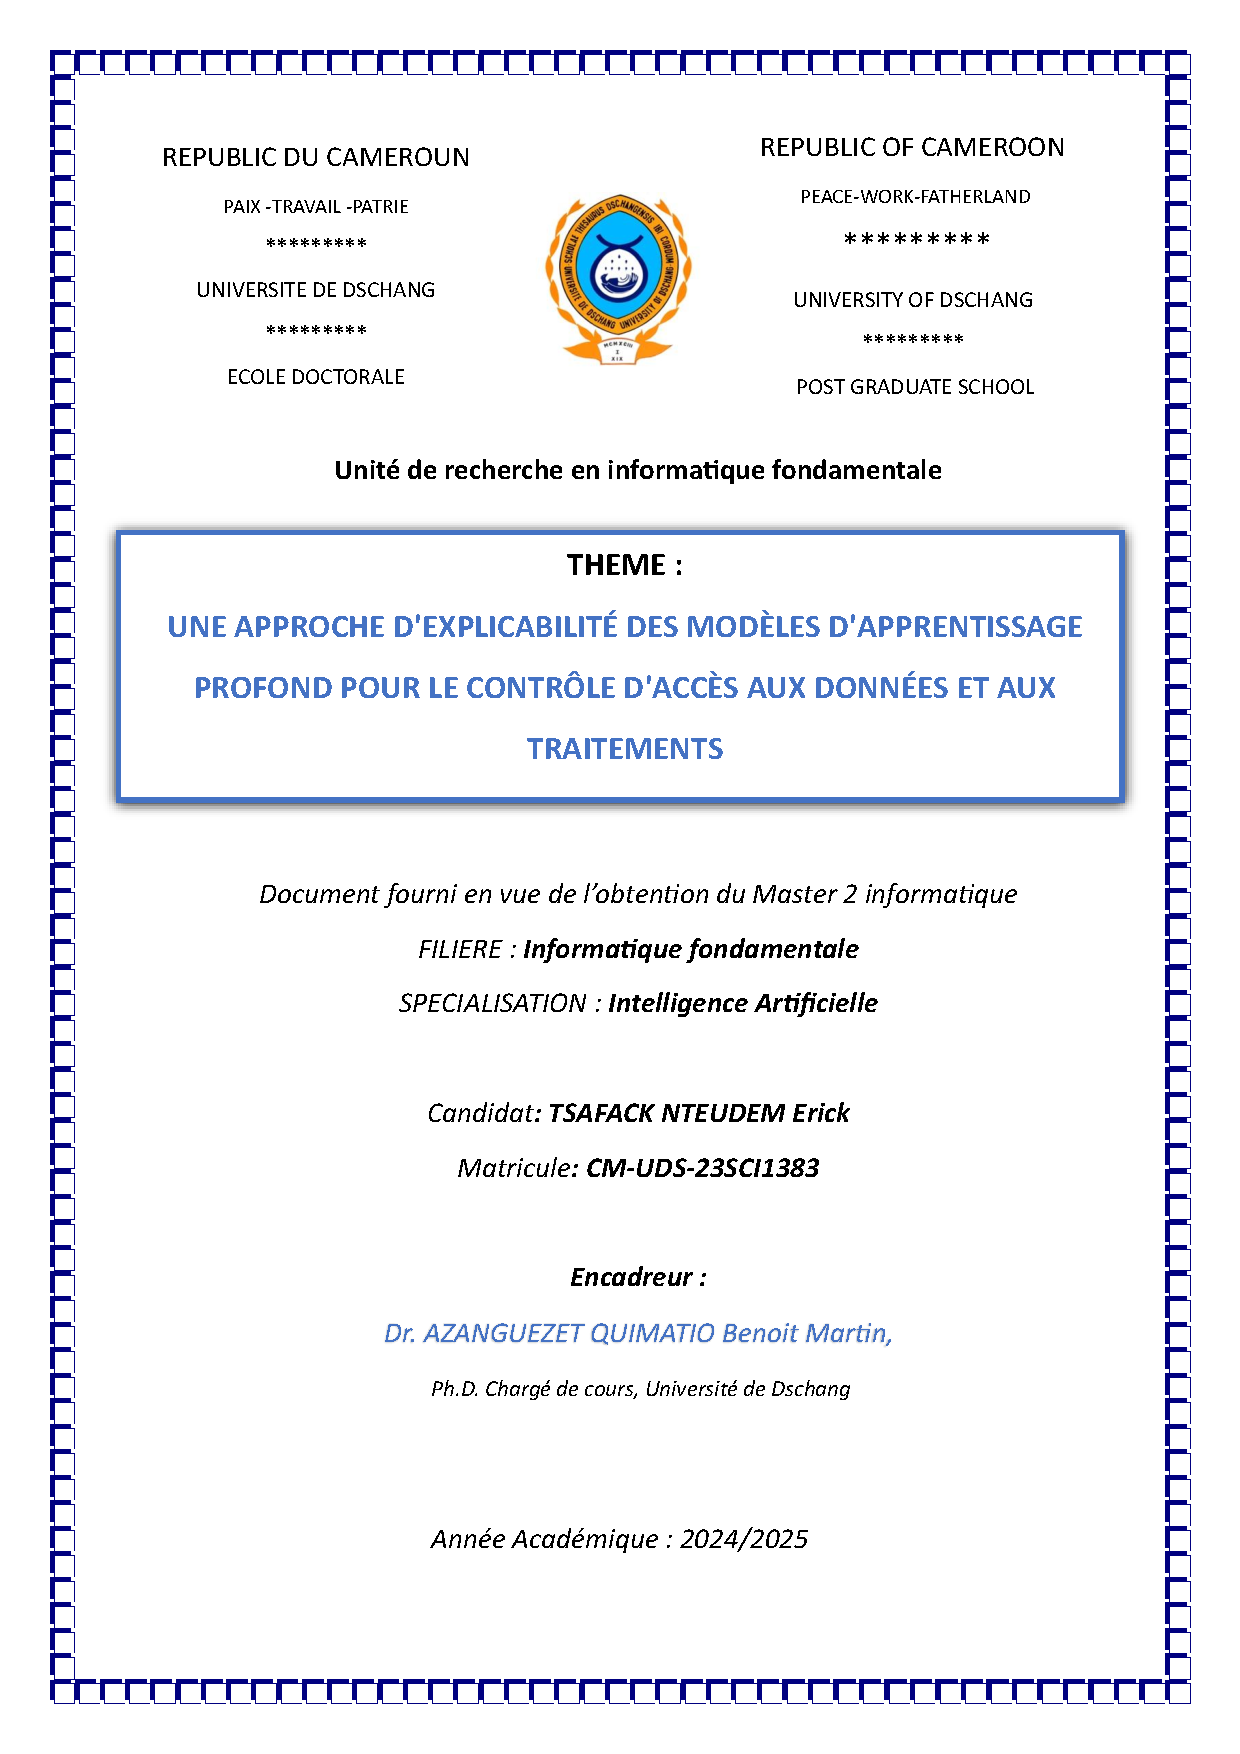
\includepdf[pages=- ,offset=2.5cm -2.5cm, trim=0.5cm 0.5cm 0.5cm 0.5cm]{Couverture_Memoire_Tsafack_Erick.pdf}
	\timesContentFontSize
    
        % 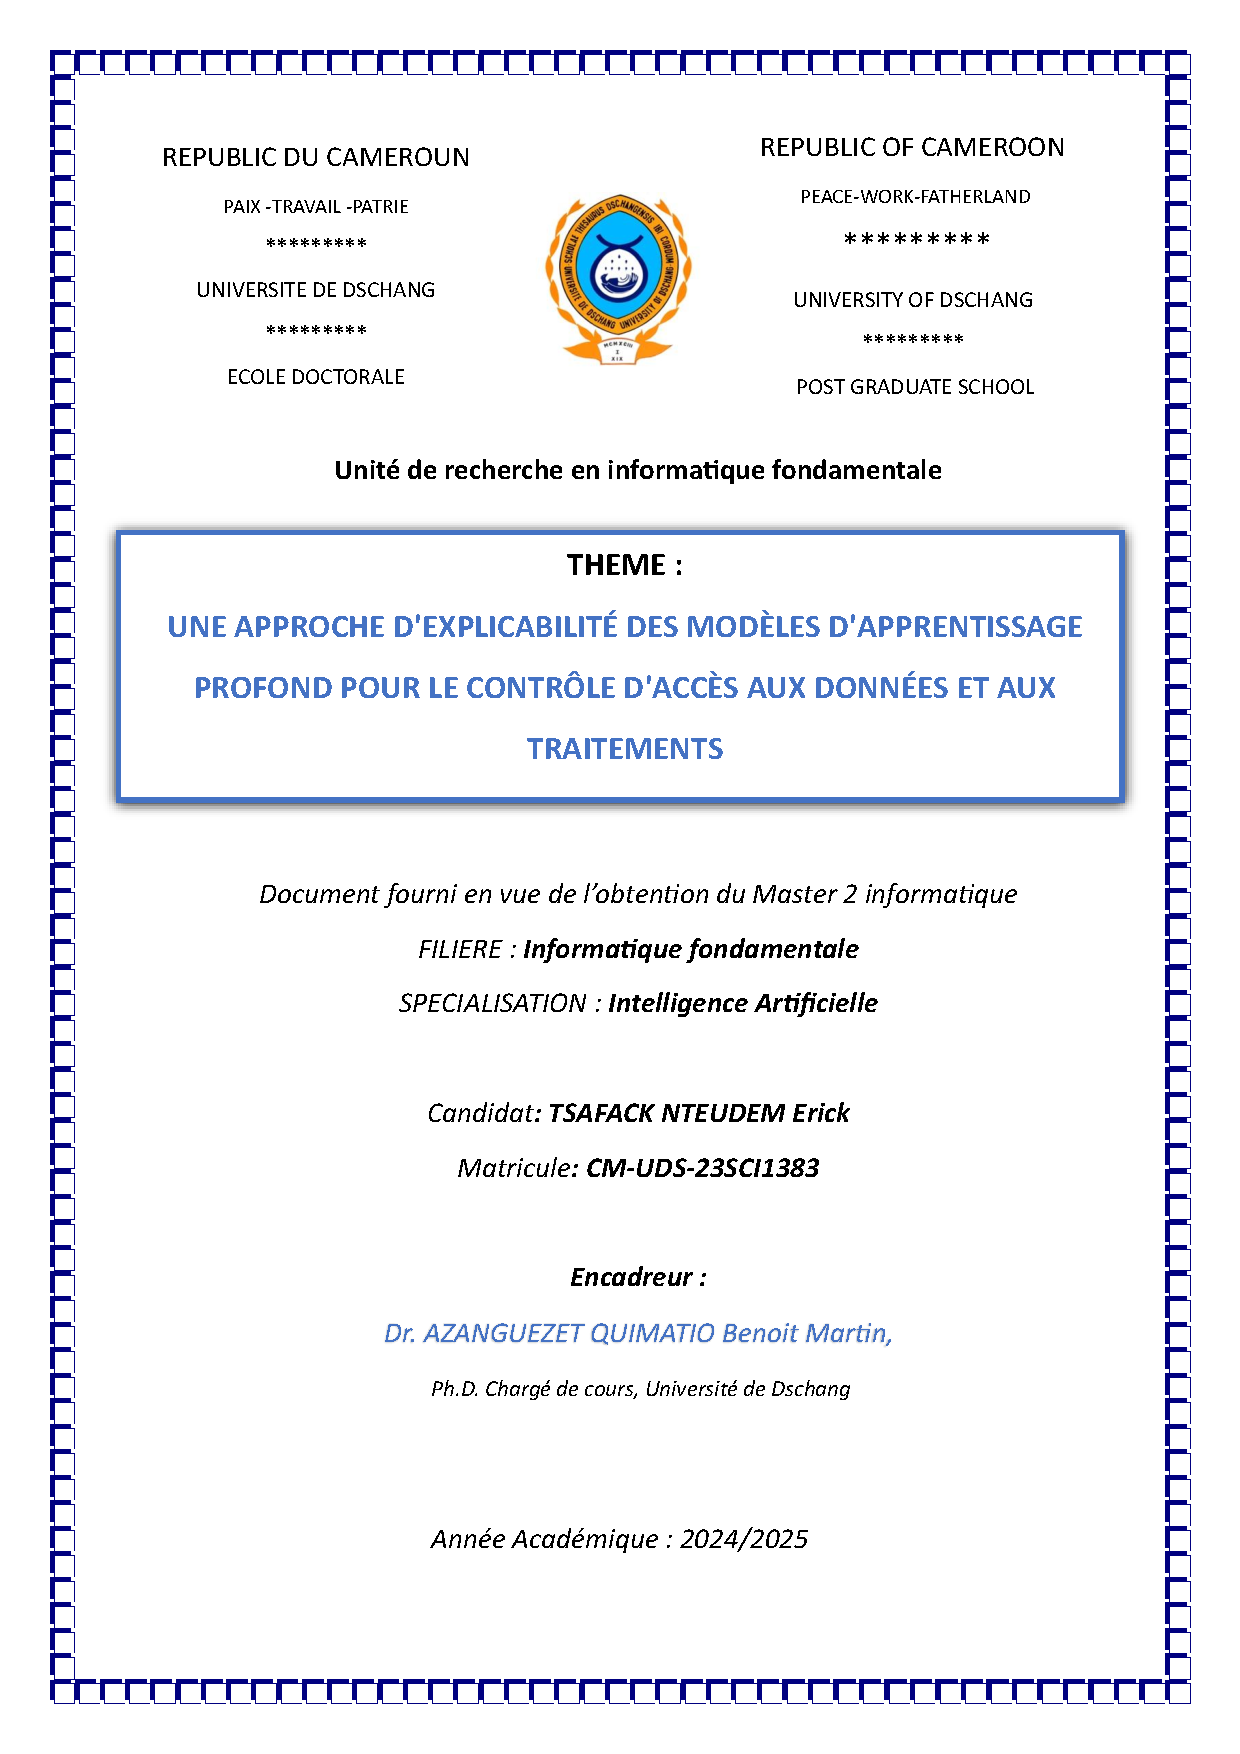
\includepdf[pages=-, scale=0.8]{Couverture_Memoire_Tsafack_Erick.pdf}
	% Code pour inclure des documents au format PDF
	%\includepdf[pages=-, offset=72 -72]{Couverture.pdf} %Insertion de la couverture
	%\includepdf[pages=-, offset=72 -72]{Originalite.pdf} %Attestation d'originalité
	%\includepdf[pages=-, offset=72 -72]{Correction.pdf} %Attestaion de correction

	\pagestyle{ruled}
	\nouppercaseheads
	\normalfont
	
            
	\frontmatter
	
	% Inclusion des fichiers de dédicaces et de remerciements
        
	%\myChapterStar{Titre}{Titre court}{Ajouter à la table des matières? (false|true|chapter|section|subsection|subsubsection -chapter par défaut-)}
\myChapterStar{Declaration of Authorship}{}{false}




	%\myChapterStar{Titre}{Titre court}{Ajouter à la table des matières? (false|true|chapter|section|subsection|subsubsection -chapter par défaut-)}
\myChapterStar{Dédicaces}{}{section}
\vspace*{7cm}
\begin{center}
\noindent \textit{\uppercase{à} mon père \textsc{NTEUDEM Henri} et à ma mère \textsc{SONGFACK Marie Christine}}.
\end{center}

\myCleanStarChapterEnd

	%\myChapterStar{Titre}{Titre court}{Ajouter à la table des matières? (false|true|chapter|section|subsection|subsubsection -chapter par défaut-)}
\myChapterStar{Remerciements}{}{section}


\myCleanStarChapterEnd

	
	% Génération de la table des matières (avec "Table of Contents" comme titre), de la liste des symboles, de la liste des acronymes, de la liste des tableaux et de la liste des figures
	% Des alternatives à ces commandes sont dispos: il suffit juste d'ajouter le suffixe "Star" pour ne pas les mettre dans la table de matière
	\myTableOfContents{Table of Contents}
	\myListOfSymbols{}
	\myListOfAcronyms{}
	\myListOfTables{}
	\myListOfFigures{}
	
	% Resumé et abstract
	\let\oldprintchaptertitle=\printchaptertitle
\renewcommand{\printchaptertitle}[1]{%
	\vspace*{-75pt}
	\oldprintchaptertitle{#1}
}%
\myChapterStar{Résumé}{}{section}
\let\printchaptertitle=\oldprintchaptertitle
% Le travail réalisé dans ce mémoire...

\vspace{1cm}
% \noindent\textbf{Mots clés:} Documents structur\'es, Workflow d'édition Coop\'erative,  Fusion des r\'epliques partielles, Conflits, Consensus, Automates d'arbre, Produit d'automates,  Évaluation paresseuse, TinyCE v2.

\myCleanStarChapterEnd

	\myChapterStar{}{}{false}
\begin{center}
\chaptitlefont %\hrule height 1.5pt
\begin{center}\textcolor{black}{\textsc{An Explainability Approach to Deep Learning Models for Data and Process Access Control}}
\end{center}
\end{center}
\vspace{8mm}
\textcolor{black}{\hrule height 4.5pt}%
\vspace{1mm}
\textcolor{black}{\hrule height 1.5pt}
	\let\oldprintchaptertitle=\printchaptertitle
\renewcommand{\printchaptertitle}[1]{%
	\vspace*{-75pt}
	\oldprintchaptertitle{#1}
}%
\myChapterStar{Abstract}{}{section}
\let\printchaptertitle=\oldprintchaptertitle
% The work presented ...

\vspace{1cm}
% \noindent\textbf{Keywords:} Structured documents, Worflow of cooperative edition, Merging partial replicas, Conflict, Consensus, Tree automata, Automata product, Lazy evaluation, TinyCE v2.

\myCleanStarChapterEnd

	\clearpage
        % \input{}
	
	% *********** Partie principale ***********
	\mainmatter
	
	% Inclusion des différents chapitres
	%\myChapterStar{Titre}{Titre court}{Ajouter à la table des matières? (false|true|chapter|section|subsection|subsubsection -chapter par défaut-)}


\myChapterStar{Introduction}{}{true}
\myMiniToc{}{Sommaire}

\mySectionStar{Contexte et Motivation}{}{true}
L'avènement des modèles d'apprentissage profond (\textit{deep learning}) a transformé de nombreux secteurs, y compris la cybersécurité, où ils sont de plus en plus utilisés pour des applications telles que le contrôle d'accès aux données et aux traitements. Ces modèles, grâce à leur capacité à traiter des volumes massifs de données et à identifier des motifs complexes, offrent une alternative puissante aux systèmes traditionnels de gestion des accès. Cependant, leur nature intrinsèquement complexe et leur manque de transparence, souvent qualifié de "boîte noire", posent des obstacles significatifs à leur adoption dans des environnements critiques où la responsabilité, la confiance et la conformité réglementaire sont essentielles \cite{zhang2022xai}. Par exemple, dans le cadre du contrôle d'accès, une décision erronée ou non justifiée peut entraîner des violations de sécurité, des fuites de données ou des atteintes à la vie privée, ce qui compromet la confiance des parties prenantes.

De plus, les réglementations modernes, telles que le Règlement Général sur la Protection des Données (RGPD) en Europe, imposent des exigences strictes en matière de transparence et d'explicabilité. L'article 22 du RGPD, par exemple, stipule que les individus ont le droit de ne pas être soumis à des décisions automatisées sans une explication adéquate \cite{goodman2017gdpr}. Cette exigence légale souligne l'importance de développer des approches qui non seulement produisent des décisions précises, mais permettent également de comprendre les raisons sous-jacentes à ces décisions. Dans ce contexte, l'\textit{Explainable Artificial Intelligence} (XAI) émerge comme une discipline clé pour combler cet écart, en proposant des méthodes et des outils capables de rendre les modèles d'apprentissage profond interprétables sans sacrifier leurs performances \cite{barredo2020xai}. Des outils comme SHAP (\textit{Shapley Additive Explanations}) \cite{lundberg2017shap} et LIME (\textit{Local Interpretable Model-agnostic Explanations}) \cite{ribeiro2016lime} ont démontré leur efficacité pour expliquer les prédictions de modèles complexes dans divers domaines. Cependant, leur application spécifique au domaine du contrôle d'accès reste largement sous-explorée, notamment pour des cas d'usage critiques comme la détection d'accès non autorisés, l'audit des permissions ou la gestion des identités numériques \cite{ahmed2021xai}. Ce manque d'approches adaptées motive la nécessité de développer des solutions XAI sur mesure pour répondre aux besoins uniques du contrôle d'accès basé sur l'apprentissage profond.



% Defining the problematic section with the provided notation
\mySectionStar{Problématique}{}{true}
Les systèmes traditionnels de contrôle d'accès, tels que le \textit{Role-Based Access Control} (RBAC) ou l'\textit{Attribute-Based Access Control} (ABAC), reposent sur des règles explicites définies manuellement, offrant une interprétabilité naturelle mais une faible adaptabilité aux environnements dynamiques comme les infrastructures cloud ou les systèmes IoT. À l'inverse, les modèles basés sur l'apprentissage profond permettent une détection en temps réel des anomalies et des comportements frauduleux grâce à leur flexibilité. Cependant, leur adoption est freinée par trois défis majeurs : l'opacité des décisions, qui complique l'audit et la justification des choix effectués \cite{rudin2019stop} ; la conformité réglementaire, exigeant des explications précises et accessibles conformes à des cadres comme le RGPD \cite{goodman2017gdpr} ; et les biais potentiels dans les données d'entraînement, pouvant conduire à des décisions discriminatoires \cite{slack2020fooling}. Ces limitations soulignent un besoin critique de solutions d'explicabilité adaptées.

\textbf{Question de recherche} : Comment concevoir une approche d'explicabilité pour les modèles d'apprentissage profond appliqués au contrôle d'accès, capable de surmonter les défis d'opacité, de conformité réglementaire et de biais, tout en répondant aux besoins des parties prenantes ?

% Defining the objectives section with the provided notation
\mySectionStar{Objectifs}{}{true}
L'objectif principal de ce travail est de développer une méthodologie d'explicabilité pour les modèles de contrôle d'accès basés sur l'apprentissage profond, garantissant des décisions transparentes, conformes et équitables dans des environnements dynamiques.

\begin{itemize}
    \item \textbf{Adapter les méthodes d'explicabilité} : Modifier des algorithmes comme SHAP et LIME pour fournir des explications pertinentes dans des scénarios de contrôle d'accès, tels que la détection d'accès frauduleux ou la gestion des permissions dynamiques.
    \item \textbf{Développer un cadre d'évaluation} : Établir des métriques et protocoles pour évaluer simultanément la performance (précision, rappel) et l'explicabilité (fidélité, compréhensibilité) des modèles, assurant un équilibre entre efficacité et transparence.
    \item \textbf{Concevoir des explications conformes et accessibles} : Proposer des formats d'explication (visualisations, textes simplifiés) compréhensibles pour des utilisateurs non techniques et conformes aux exigences réglementaires, notamment celles du RGPD.
\end{itemize}


\mySectionStar{Organisation du Mémoire}{}{true}
Ce document est structuré en plusieurs chapitres pour couvrir de manière exhaustive le sujet :

\begin{itemize}
    \item \textbf{Chapitre 1 : Cadre théorique} : Présentation des concepts fondamentaux de l'\textit{Explainable AI} (XAI) et des systèmes de contrôle d'accès, ainsi qu'une analyse des exigences spécifiques des environnements critiques.
    \item \textbf{Chapitre 2 : État de l'art} : Revue détaillée des méthodes d'explicabilité existantes (SHAP, LIME, etc.) et identification de leurs limites lorsqu'elles sont appliquées au contrôle d'accès.
    \item \textbf{Chapitre 3 : Proposition méthodologique} : Développement d'une approche originale pour intégrer l'explicabilité dans les modèles de contrôle d'accès, en s'appuyant sur les lacunes identifiées dans l'état de l'art.
    \item \textbf{Chapitre 4 : Expérimentations} : Mise en œuvre de la méthodologie proposée à travers des études de cas (ex. : détection d'accès frauduleux) et analyse des résultats en termes de performance et d'explicabilité.
    \item \textbf{Chapitre 5 : Conclusion et perspectives} : Résumé des contributions, discussion des limites de l'approche proposée et suggestions pour des travaux futurs, notamment dans des domaines comme l'explicabilité en temps réel ou l'intégration avec d'autres technologies émergentes.
\end{itemize}



	\part{État des Lieux}
	%\myChapter{Titre}{Titre court}
\myChapter{Cadre Théorique}{}
\label{chapCadreTheorique}
%\myMinitoc{Profondeur de la minitoc (section|subsection|subsubsection)}{Titre de la minitoc}
\myMiniToc{section}{Sommaire}


\mySection{Introduction}{}\label{sectionintoCadretheorique}
Ce chapitre vise à poser les bases théoriques nécessaires à la compréhension des concepts centraux de ce mémoire, à savoir l'explicabilité des modèles d'apprentissage profond (\textit{deep learning}) et leur application dans le domaine du contrôle d'accès aux données et aux traitements. Il explore les principes fondamentaux de l'\textit{Explainable Artificial Intelligence} (XAI), les mécanismes des systèmes de contrôle d'accès, et les exigences spécifiques des environnements critiques où la transparence et la conformité sont essentielles. Ce chapitre fournit également un cadre conceptuel pour analyser les interactions entre ces deux domaines, en mettant en lumière les opportunités et les défis associés.



\mySection{L’Apprentissage Profond et ses Limites}{}
L’apprentissage profond (\textit{deep learning}, DL) a révolutionné de nombreux domaines grâce à sa capacité à modéliser des relations complexes dans des données volumineuses et non structurées. Cette section vise à établir les bases théoriques du DL, en explorant ses principes fondamentaux, ses applications dans des domaines critiques comme le contrôle d’accès, et les limites inhérentes à son opacité, qui freinent son adoption dans des systèmes où la transparence est essentielle \cite{jouis2020}. L’objectif est de fournir un cadre conceptuel pour comprendre pourquoi l’explicabilité est cruciale pour surmonter ces défis, en particulier dans le contexte de la cybersécurité et de la gestion des accès \cite{zhang2022xai}.

\mySubSection{Introduction à l’Apprentissage Profond}{}
L’apprentissage profond est une sous-discipline de l’apprentissage automatique qui repose sur des réseaux de neurones artificiels organisés en couches multiples, capables de traiter des données complexes sans nécessiter d’ingénierie manuelle des caractéristiques \cite{lecun2015deep}. Apparu comme une approche dominante dans les années 2010, le DL a permis des avancées majeures dans des domaines variés, tels que la reconnaissance d’images, le traitement du langage naturel, et la cybersécurité. Dans le contexte du contrôle d’accès, les modèles de DL sont de plus en plus utilisés pour détecter des anomalies, gérer des permissions dynamiques, et auditer les accès \cite{nobi2022dlbac}. Cette sous-section introduit les concepts clés du DL, met en lumière ses avantages (par exemple, l’extraction automatique de caractéristiques, la robustesse face à des données hétérogènes), et souligne son rôle croissant dans les systèmes critiques où la précision et l’adaptabilité sont primordiales \cite{barredo2020xai}.

\begin{figure}[h]
    \centering
    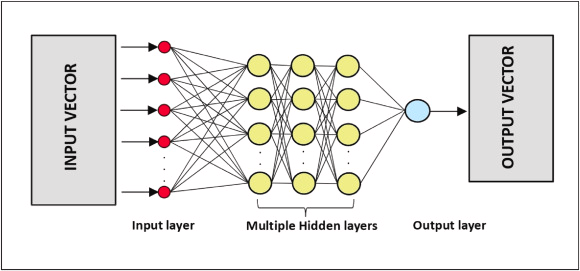
\includegraphics[width=0.8\textwidth]{My-Thesis/Chap1/images/deep_learning_model.png}
    \caption{Représentation schématique d’un réseau de neurones profond, illustrant les couches d’entrée, cachées, et de sortie, ainsi que le flux de données à travers les connexions pondérées. Cette visualisation montre la complexité des architectures de DL, qui contribue à leur puissance mais aussi à leur opacité.}
    \label{fig:dl_overview}
\end{figure}

\mySubSection{Principes Fondamentaux du Deep Learning}{}
\mySubSubSection{Architecture des Réseaux de Neurones}{}
Les réseaux de neurones profonds sont composés de multiples couches de neurones artificiels, interconnectés par des poids appris lors de l’entraînement. Chaque neurone effectue une transformation linéaire suivie d’une fonction d’activation non linéaire (par exemple, ReLU, sigmoïde), permettant au réseau de modéliser des relations complexes \cite{lecun2015deep}. Les architectures courantes incluent les réseaux convolutifs (CNN) pour les données structurées, les réseaux récurrents (RNN) pour les séquences, et les réseaux à attention pour les tâches nécessitant une focalisation sur des éléments spécifiques. Dans le contrôle d’accès, les CNN peuvent analyser des logs formatés, tandis que les RNN sont adaptés à l’analyse des historiques d’accès \cite{karpathy2015visualizing}. Cette sous-section détaille la structure des réseaux, leur modularité, et leur capacité à s’adapter à différents types de données.

\begin{figure}[h]
    \centering
    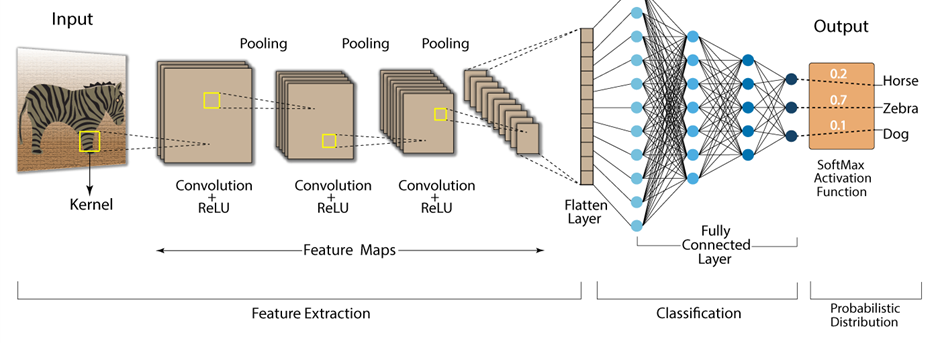
\includegraphics[width=1.0\textwidth]{My-Thesis/Chap1/images/cnn.png}
    \caption{Architecture d’un réseau convolutif (CNN), montrant les couches de convolution, de pooling, et de classification. Cette visualisation illustre comment un CNN extrait des caractéristiques hiérarchiques à partir de données.}
    \label{fig:cnn_architecture}
\end{figure}

\mySubSubSection{Processus d’Entraînement}{}
L’entraînement d’un modèle de DL repose sur la minimisation d’une fonction de perte, qui mesure l’écart entre les prédictions du modèle et les valeurs attendues. Ce processus utilise la rétropropagation du gradient pour ajuster les poids des connexions, souvent via des algorithmes d’optimisation comme la descente de gradient stochastique (SGD) ou Adam \cite{lecun2015deep}. Cette sous-section explique les étapes clés de l’entraînement, les besoins en données volumineuses et étiquetées, et les défis liés à la qualité des données, comme les biais ou les données incomplètes, qui peuvent affecter les performances dans le contrôle d’accès \cite{slack2020fooling}. Elle aborde également l’importance des hyperparamètres (taux d’apprentissage, taille des couches) et des ressources computationnelles nécessaires.

\mySubSubSection{Types de Modèles de Deep Learning}{}
Cette sous-section présente les modèles de DL les plus pertinents pour le contrôle d’accès :
\begin{itemize}
    \item \textbf{Réseaux Convolutifs (CNN)} : Utilisés pour traiter des données structurées, comme les images ou les logs d’accès formatés. Les CNN extraient des motifs spatiaux, utiles pour détecter des anomalies dans les métadonnées d’accès \cite{selvaraju2017gradcam}.
    \item \textbf{Réseaux Récurrents (RNN) et LSTM} : Conçus pour les données séquentielles, comme les historiques d’accès, permettant de modéliser des comportements temporels \cite{karpathy2015visualizing}.
    \item \textbf{Réseaux à Attention} : Ces modèles, comme les transformers, mettent en évidence les attributs critiques (par exemple, localisation ou heure) dans les décisions d’accès \cite{lin2017structured}.
\end{itemize}
Chaque type est illustré par son application potentielle dans le contrôle d’accès, avec un accent sur leur adaptabilité aux environnements dynamiques.

\mySubSection{Applications du Deep Learning dans le Contrôle d’Accès}{}
Le DL offre des solutions puissantes pour moderniser les systèmes de contrôle d’accès, surpassant souvent les approches traditionnelles comme le \textit{Role-Based Access Control} (RBAC) ou l’\textit{Attribute-Based Access Control} (ABAC) \cite{sandhu1996role, hu2013abac}. Cette section explore trois applications clés :
\begin{itemize}
    \item \textbf{Détection d’anomalies} : Les modèles de DL, comme les autoencodeurs ou les RNN, identifient des comportements d’accès inhabituels, tels que des tentatives d’intrusion ou des connexions depuis des localisations non autorisées \cite{nobi2022dlbac}.
    \item \textbf{Gestion dynamique des permissions} : Les réseaux à attention permettent d’adapter les droits d’accès en temps réel en fonction de contextes complexes, comme l’heure, le lieu, ou le type de dispositif \cite{lin2017structured}.
    \item \textbf{Audit des accès} : Les CNN ou LSTM analysent les historiques pour détecter des violations potentielles, offrant une alternative automatisée aux audits manuels \cite{ahmed2021xai}.
\end{itemize}
Des exemples concrets, comme l’utilisation de LSTM pour modéliser des séquences de connexions, sont discutés, avec une comparaison des avantages du DL (flexibilité, précision) et des défis liés à son opacité.


\begin{figure}[h]
    \centering
    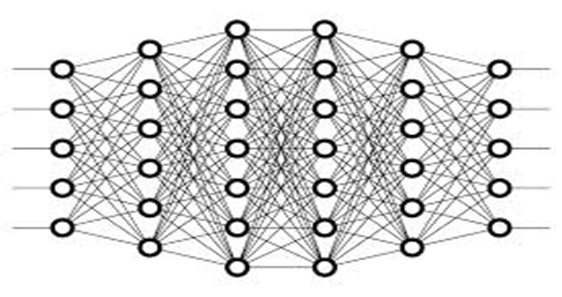
\includegraphics[width=0.8\textwidth]{My-Thesis/Chap1/images/lstm.png}
    \caption{Réseau de neurone complexe.}
    \label{fig:lstm_sequence}
\end{figure}

\mySubSection{Limites du Deep Learning}{}
\mySubSubSection{Opacité des Modèles}{}
Les modèles de DL sont souvent qualifiés de « boîtes noires » en raison de leur complexité architecturale et du grand nombre de paramètres (parfois des millions) \cite{rudin2019stop}. Cette opacité rend difficile l’interprétation des décisions, ce qui pose problème dans le contrôle d’accès, où les administrateurs doivent justifier les refus ou les autorisations d’accès. Cette sous-section explore les raisons techniques de cette opacité, comme la non-linéarité des fonctions d’activation et l’interdépendance des couches, et leurs implications pour la confiance des utilisateurs \cite{jouis2020}.

\mySubSubSection{Biais et Discriminations}{}
Les modèles de DL peuvent hériter ou amplifier des biais présents dans les données d’entraînement, entraînant des décisions discriminatoires, comme le refus d’accès basé sur des corrélations démographiques non pertinentes \cite{slack2020fooling}. Cette partie examine les sources de biais (données déséquilibrées, étiquettes erronées) et leur impact dans le contrôle d’accès, ainsi que les défis pour les détecter et les corriger sans outils d’explicabilité adaptés.

\mySubSubSection{Conformité aux Réglementations}{}
Les réglementations, comme l’article 22 du RGPD, exigent que les décisions automatisées soient accompagnées d’explications compréhensibles \cite{goodman2017gdpr}. Cette sous-section analyse les obstacles à la production d’explications conformes avec les modèles de DL, en raison de leur complexité et de l’absence de méthodes d’explicabilité standardisées. Elle discute des implications pour les systèmes de contrôle d’accès, où la conformité est cruciale \cite{desmoulin2019}.

% \begin{figure}[h]
%     \centering
%     \includegraphics[width=0.8\textwidth]{bias_visualization.png}
%     \caption{Représentation des biais dans un modèle de DL pour le contrôle d’accès, montrant comment des corrélations non pertinentes (par exemple, démographiques) peuvent influencer une décision de refus d’accès. Cette visualisation met en évidence la nécessité d’outils d’explicabilité pour détecter ces biais.}
%     \label{fig:bias_visualization}
% \end{figure}

\mySubSection{Nécessité de l’Explicabilité}{}
Face aux limites du DL, l’\textit{Explainable Artificial Intelligence} (XAI) émerge comme une solution pour rendre les modèles plus transparents et conformes. Cette section introduit les principales méthodes d’explicabilité, telles que LIME (approximation linéaire locale), SHAP (valeurs de Shapley), et les mécanismes d’attention, qui permettent de justifier les décisions des modèles \cite{ribeiro2016lime, lundberg2017shap, lin2017structured}. Elle souligne leur pertinence pour le contrôle d’accès, où les explications doivent être à la fois précises, compréhensibles, et conformes aux exigences légales \cite{barredo2020xai}. Une discussion sur l’équilibre entre performance et explicabilité conclut cette partie.

\mySubSection{Conclusion de la Section}{}
Cette section a exploré les principes fondamentaux, les applications, et les limites de l’apprentissage profond, en mettant l’accent sur son rôle dans le contrôle d’accès. Si le DL offre une puissance et une flexibilité inégalées, son opacité, ses biais potentiels, et les défis de conformité réglementaire nécessitent des approches d’explicabilité robustes. Ces concepts préparent le terrain pour les sections suivantes, qui analyseront les méthodes d’explicabilité et les systèmes de contrôle d’accès traditionnels et basés sur l’IA.



\mySection{L'Explainable Artificial Intelligence (XAI)}{}\label{sectionXAICadre}

\mySubSection{Introduction à l’XAI}{}\label{xaiIntro}
L'\textit{Explainable Artificial Intelligence} (XAI), ou intelligence artificielle explicable, émerge comme une discipline clé visant à rendre les modèles d'intelligence artificielle compréhensibles pour les humains. Cette nécessité découle de l'opacité inhérente à de nombreux modèles, notamment ceux basés sur l'apprentissage profond, souvent qualifiés de "boîtes noires" en raison de la difficulté à interpréter leurs processus décisionnels \cite{jouis2020}. L'explicabilité est particulièrement cruciale dans des contextes où la transparence et la confiance sont essentielles, comme le contrôle d'accès aux données et aux traitements. Dans ce domaine, une décision non justifiée peut entraîner des conséquences graves, telles que des violations de sécurité ou des atteintes à la vie privée. L'essor récent de l'XAI, motivé par ces limites, s'inscrit dans une volonté de répondre aux attentes des utilisateurs et aux exigences réglementaires, tout en maintenant les performances des modèles \cite{jouis2020}.

\mySubSection{Définitions et Objectifs de l’XAI}{}
L'explicabilité peut être définie comme la capacité d'un modèle à fournir des explications compréhensibles par un humain, que ce soit en décrivant son fonctionnement global ou en justifiant une décision spécifique \cite{miller2019explanation}. Cette transparence vise à permettre aux utilisateurs, qu'ils soient experts ou non, de comprendre les raisons sous-jacentes aux prédictions ou aux décisions automatisées. Les objectifs principaux de l'XAI incluent l'amélioration de la confiance des utilisateurs envers les systèmes intelligents, la facilitation de l'audit des modèles pour détecter d'éventuels biais ou erreurs, et la conformité aux exigences légales et éthiques, telles que celles imposées par le Règlement Général sur la Protection des Données (RGPD) \cite{gilpin2018explaining}. Une distinction fondamentale est faite entre l'explicabilité globale, qui cherche à comprendre le comportement général du modèle, et l'explicabilité locale, qui se concentre sur l'explication d'une décision particulière pour une instance donnée \cite{ribeiro2016lime}.



\mySubSection{Taxonomie des Méthodes d’Explicabilité}{}
Les méthodes d'explicabilité des modèles d'apprentissage profond peuvent être classées en trois grandes catégories en fonction de leur niveau de transparence vis-à-vis de la structure interne du modèle \cite{jouis2020, guidotti2018}. Cette taxonomie, illustrée dans la littérature par des approches variées, permet de structurer les techniques selon qu'elles traitent le modèle comme une boîte noire, une boîte grise ou une boîte blanche. Chaque catégorie répond à des contraintes techniques et à des besoins spécifiques des utilisateurs, qu’il s’agisse de simplicité, de fidélité au modèle ou de compréhensibilité. La figure~\ref{fig:taxonomie_xai} illustre schématiquement ces trois approches en fonction de leur dépendance à l'architecture du modèle et de leur niveau d'interprétabilité.

\begin{figure}[h]
    \centering
    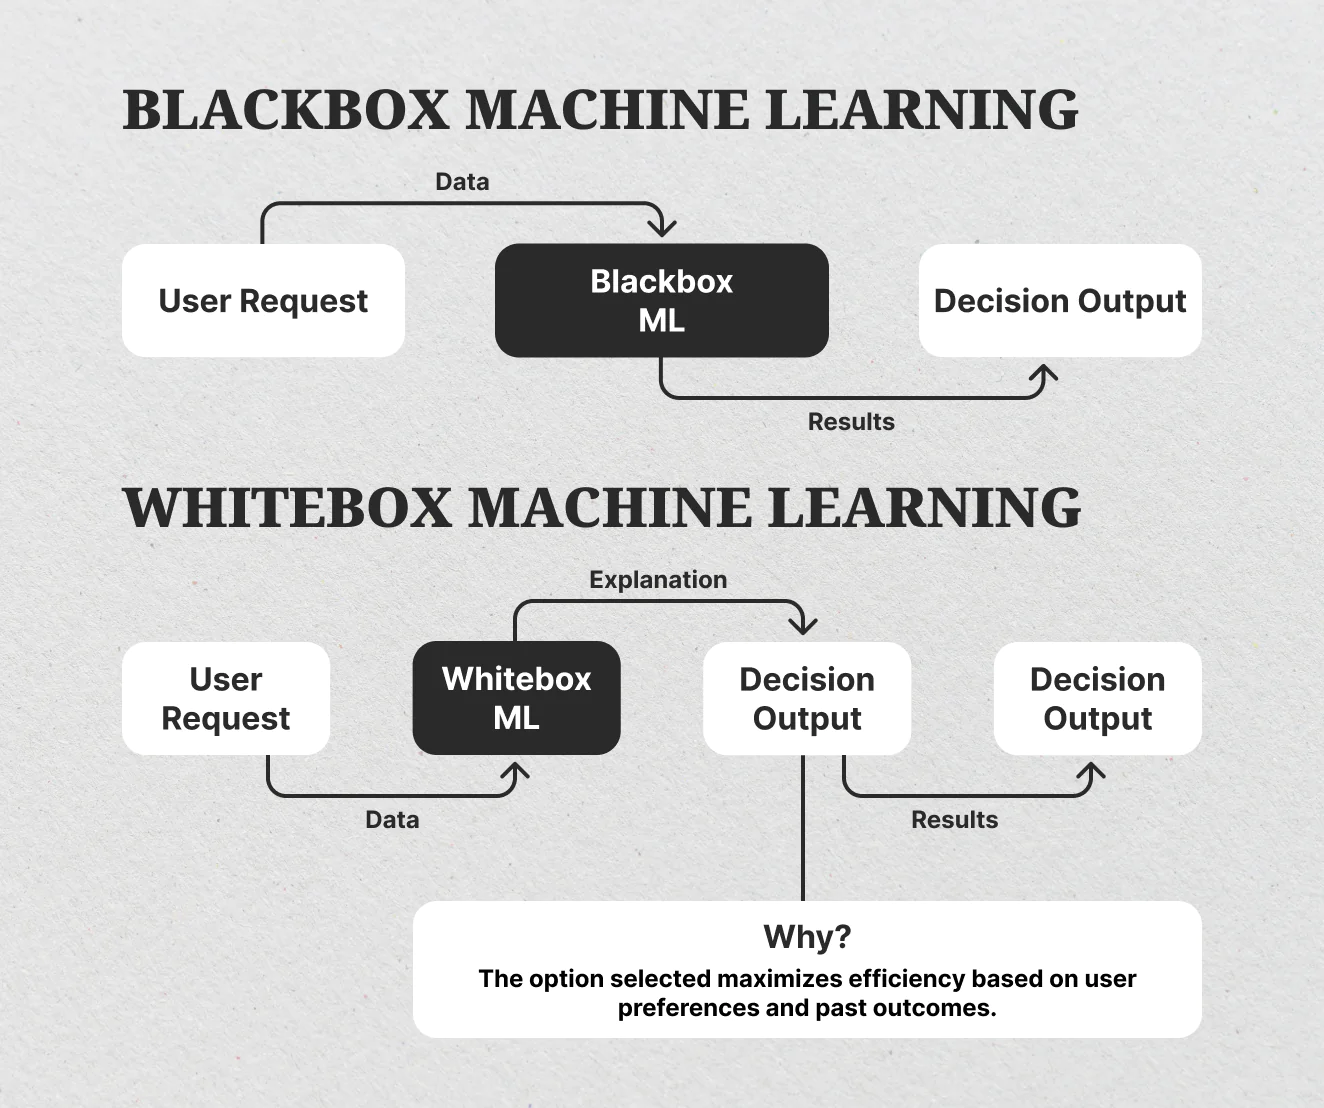
\includegraphics[width=0.8\textwidth]{My-Thesis/Chap1/images/taxonomy.png}
    \caption{Taxonomie des méthodes d'explicabilité : boîte noire (indépendante du modèle), et boîte blanche (modèle interprétable). L'axe vertical représente le niveau d'interprétabilité}
    \label{fig:taxonomie_xai}
\end{figure}

\begin{itemize}
    \item \textbf{Approches indépendantes du modèle (boîte noire)} : Ces méthodes analysent les entrées et sorties du modèle sans accéder à sa structure interne. Elles sont flexibles, car applicables à tout type de modèle, mais reposent souvent sur des corrélations plutôt que sur des causalités. Par exemple, des outils comme LIME ou SHAP quantifient l'impact des variables d'entrée sur les prédictions \cite{guidotti2018}. Elles sont particulièrement adaptées lorsque la priorité est de fournir des explications rapides et générales, sans nécessiter une expertise approfondie de l'architecture sous-jacente. Cependant, leur fidélité peut être limitée, car elles ne capturent pas toujours les mécanismes précis du modèle.
    % \begin{figure}
    %     \centering
    %     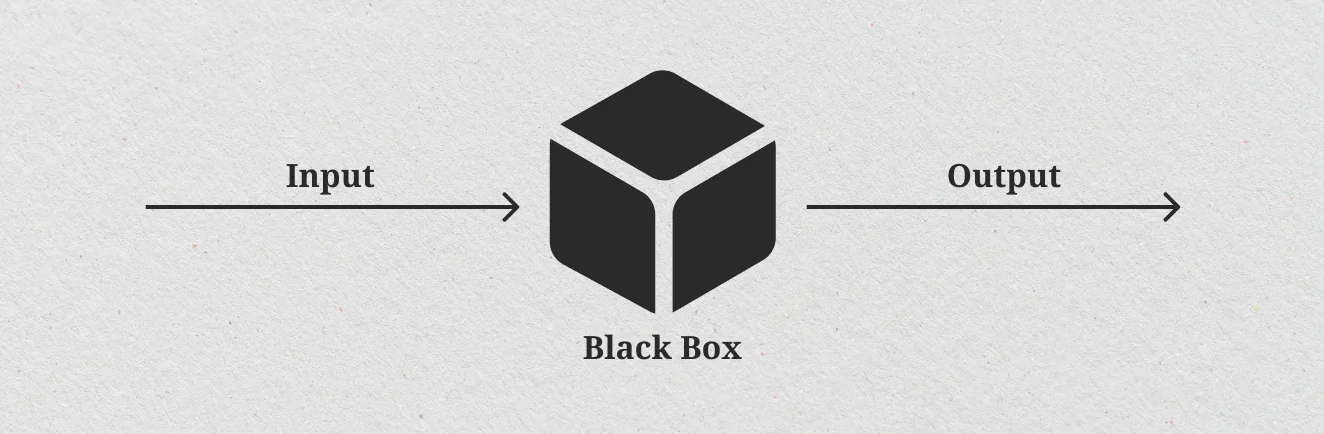
\includegraphics[width=0.6\linewidth]{chap1//images/blackbox_ai.png}
    %     \caption{modele boite noire}
    %     \label{fig:enter-label}
    % \end{figure}

    \item \textbf{Approches dépendantes du modèle (boîte grise)} : Ces techniques exploitent les paramètres internes du modèle, comme les poids des neurones ou les activations des couches, pour générer des explications. Elles offrent une meilleure fidélité, car elles reflètent directement le fonctionnement du modèle, mais sont contraintes par l'architecture spécifique (par exemple, CNN ou LSTM) \cite{jouis2020}. Des méthodes comme Grad-CAM, qui produit des cartes de chaleur pour les réseaux convolutifs, permettent de visualiser les régions influentes d’une entrée \cite{selvaraju2017gradcam}. Ces approches conviennent aux scénarios où une compréhension fine du modèle est nécessaire, mais elles exigent des compétences techniques pour interpréter les résultats.

    \item \textbf{Modèles interprétables (boîte blanche)} : Ces approches intègrent l'explicabilité dès la conception du modèle, en utilisant des architectures intrinsèquement transparentes, comme les mécanismes d'attention ou des réseaux simplifiés \cite{jouis2020}. Elles garantissent une compréhensibilité élevée, car les explications sont directement dérivées des paramètres du modèle, mais peuvent sacrifier une partie des performances par rapport aux modèles complexes. Elles sont idéales pour les applications où la transparence est une priorité absolue, comme dans les systèmes critiques soumis à des réglementations strictes.

\end{itemize}

Chaque catégorie présente des avantages et des limites, qui dépendent des contraintes du projet et des attentes des utilisateurs. Par exemple, dans le cadre du contrôle d'accès, les approches indépendantes du modèle peuvent être privilégiées pour leur flexibilité, tandis que les modèles interprétables sont mieux adaptés pour répondre aux exigences légales de transparence, comme celles imposées par le RGPD \cite{guidotti2018}. Le choix d’une méthode doit donc équilibrer la fidélité des explications, leur compréhensibilité et les ressources disponibles pour leur mise en œuvre.





\mySubSection{Méthodes Spécifiques d’Explicabilité}{}

Cette section détaille les principales méthodes d'explicabilité utilisées pour rendre les modèles d'apprentissage profond plus transparents, en se concentrant sur leur application potentielle au contrôle d'accès. Ces approches sont classées en trois catégories selon leur dépendance à l'architecture du modèle : approches indépendantes du modèle, approches dépendantes du modèle, et modèles interprétables. Chaque méthode est illustrée, lorsque pertinent, par des visualisations issues de la littérature.

\mySubSubSection{Approches indépendantes du modèle}{}

Les approches indépendantes du modèle, souvent qualifiées d'agnostiques, permettent d'expliquer les prédictions sans nécessiter une connaissance approfondie de la structure interne du modèle. Elles se basent principalement sur l'analyse des relations entre les entrées et les sorties, offrant ainsi une grande flexibilité d'application.

\paragraph{LIME (Local Interpretable Model-agnostic Explanations)}  
L'outil LIME, proposé par \cite{ribeiro2016lime}, génère des explications locales en approximant le comportement d'un modèle complexe autour d'une instance spécifique à l'aide d'un modèle linéaire simple. Pour une prédiction donnée, LIME identifie les variables d'entrée ayant le plus d'impact, comme les mots dans un texte ou les pixels dans une image, et quantifie leur influence positive ou négative sur la décision. Cette méthode est particulièrement utile pour expliquer des décisions dans des contextes comme le contrôle d'accès, où il peut être nécessaire de justifier pourquoi un accès a été refusé en mettant en évidence des facteurs clés (par exemple, une tentative d'accès à une heure inhabituelle).  

\begin{figure}[h]
    \centering
    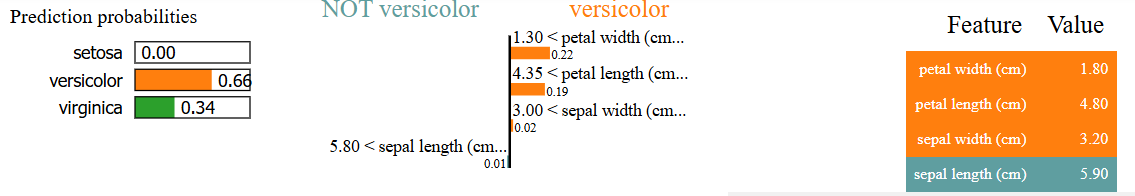
\includegraphics[width=0.8\textwidth]{My-Thesis/Chap1/images/lime_explanation.png}
    \caption{LIME : Visualisation de l’importance des mots dans une prédiction textuelle, où chaque mot est associé à un poids reflétant son influence sur la classe prédite \citep{ribeiro2016why}.}
    \label{fig:lime}
\end{figure}

\paragraph{Ancres}  
Les Ancres, une amélioration de LIME proposée par \citet{ribeiro2018anchors}, fournissent des explications sous forme de règles logiques définissant le contexte dans lequel une prédiction est valide. Par exemple, pour une décision de contrôle d'accès, une ancre pourrait être : "Si l’utilisateur tente d’accéder depuis un emplacement non autorisé et à une heure inhabituelle, alors l’accès est refusé." Ces règles sont construites pour maximiser la précision (fidélité au modèle) et la couverture (généralisation à d’autres instances similaires). Cette approche est particulièrement adaptée pour des systèmes nécessitant des justifications claires et compréhensibles par des utilisateurs non techniques.

\begin{figure}[h]
    \centering
    \includegraphics[width=0.8\textwidth]{My-Thesis/Chap1/images/anchor_explanation.png}
    \caption{Anchor : Visualisation des parties importantes d’une entrée (par exemple, mots ou régions d’image) définissant une règle d’explication pour une prédiction spécifique \citep{ribeiro2018anchors}.}
    \label{fig:anchor}
\end{figure}

\paragraph{Valeurs de Shapley et SHAP}  
Inspirées de la théorie des jeux, les valeurs de Shapley quantifient la contribution de chaque variable d’entrée à une prédiction \citep{lundberg2017shap}. Le module SHAP (\textit{Shapley Additive Explanations}) optimise ce calcul pour le rendre applicable à des modèles complexes, en fournissant une mesure de l’importance des variables sous forme de scores additifs. Par exemple, dans le cadre du contrôle d’accès, SHAP pourrait révéler qu’une tentative d’accès a été refusée principalement en raison de l’historique des connexions de l’utilisateur. Cependant, cette méthode peut être difficile à interpréter pour des utilisateurs non experts en raison de la complexité des calculs et de la nécessité d’un post-traitement pour simplifier les résultats.

\paragraph{Limites}  
Les approches indépendantes du modèle, bien que flexibles, présentent des limites. Elles mettent en évidence des corrélations entre entrées et sorties, mais ne garantissent pas une compréhension causale des décisions. De plus, leur complexité peut rendre les explications difficiles à assimiler pour des utilisateurs sans expertise technique, en particulier dans des domaines comme le contrôle d’accès où les explications doivent être conformes aux réglementations.

\mySubSubSection{Approches dépendantes du modèle}{}

Les approches dépendantes du modèle exploitent la structure interne du modèle pour générer des explications plus fidèles à son fonctionnement. Elles nécessitent une connaissance de l’architecture, ce qui limite leur applicabilité mais améliore leur précision.

\paragraph{Grad-CAM}  
La méthode Grad-CAM (\textit{Gradient-weighted Class Activation Mapping}), proposée par \cite{selvaraju2017gradcam}, génère des cartes de chaleur pour visualiser les régions d’une entrée (généralement une image) influençant une prédiction dans un réseau convolutif (CNN). Bien que principalement utilisée pour l’analyse d’images, cette méthode pourrait être adaptée au contrôle d’accès pour des données visuelles, comme des captures d’écran de tentatives d’accès frauduleuses, en mettant en évidence les zones critiques de l’image. La fidélité de Grad-CAM à la décision du modèle en fait un outil puissant, mais son application est restreinte aux architectures convolutives.


\begin{figure}[h]
    \centering
    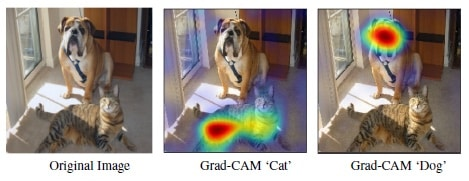
\includegraphics[width=0.8\textwidth]{My-Thesis/Chap1/images/gradcam_visualization.png}
    \caption{Visualisation d'une explication Grad-CAM.}
    \label{fig:gradcam}
\end{figure}

dans la figure \ref{fig:gradcam}, la Carte de chaleur met en évidence les régions d’une image influençant la classification dans un réseau convolutif, comme les zones pertinentes pour identifier une classe spécifique, l'un pour les chiens et l'autre pour les chats. \citep{GradCAMImage}

\paragraph{Analyse des LSTM}  
Les réseaux Long Short-Term Memory (LSTM) sont largement utilisés pour l’analyse de séquences, comme les logs d’accès dans un système de contrôle. \citet{karpathy2015visualizing} proposent d’étudier les activations des cellules LSTM pour comprendre les motifs détectés, comme la reconnaissance de motifs spécifiques dans un texte (par exemple, des guillemets indiquant une citation). Dans le contexte du contrôle d’accès, cette méthode pourrait révéler pourquoi un modèle a identifié une séquence d’actions comme suspecte. Cependant, l’analyse des activations est complexe et nécessite une exploration approfondie, ce qui peut limiter son accessibilité.


\begin{figure}[h]
    \centering
    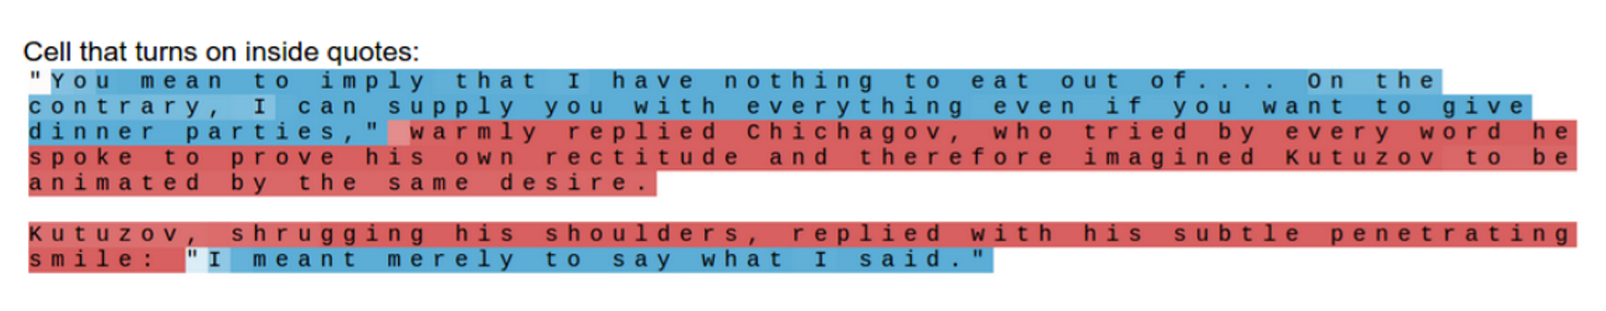
\includegraphics[width=0.8\textwidth]{My-Thesis/Chap1/images/lstm_activation.png}
    \caption{Activation d’une cellule en fonction des guillemets dans le texte : Visualisation des activations d’une cellule LSTM détectant des motifs textuels spécifiques, comme les guillemets \citep{karpathy2015visualizing}.}
    \label{fig:lstm}
\end{figure}

\paragraph{Avantages et inconvénients}  
Les approches dépendantes du modèle offrent une grande fidélité, car elles s’appuient directement sur les mécanismes internes du modèle. Elles sont particulièrement utiles pour des experts souhaitant auditer un système de contrôle d’accès. Cependant, leur dépendance à l’architecture limite leur généralisation, et leur complexité peut poser des défis pour des explications destinées à des utilisateurs non techniques.

\mySubSubSection{Modèles interprétables}{}

Les modèles interprétables, ou boîtes blanches, sont conçus pour être transparents par leur architecture, réduisant ainsi le besoin d’analyses post-entraînement.

\paragraph{Mécanismes d’attention}  
Les mécanismes d’attention, décrits par \cite{lin2017structured}, permettent de visualiser les poids attribués aux différentes parties d’une entrée, comme les mots dans une phrase. Dans une tâche de traduction, par exemple, les poids d’attention mettent en évidence les correspondances entre mots source et cible. Appliqués au contrôle d’accès, ces mécanismes pourraient identifier les éléments clés d’une requête d’accès (par exemple, un identifiant utilisateur ou une adresse IP) influençant la décision. Cette approche est intuitive et ne nécessite pas de calculs supplémentaires après l’entraînement, mais elle est spécifique aux modèles intégrant une couche d’attention.



\begin{figure}[h]
    \centering
    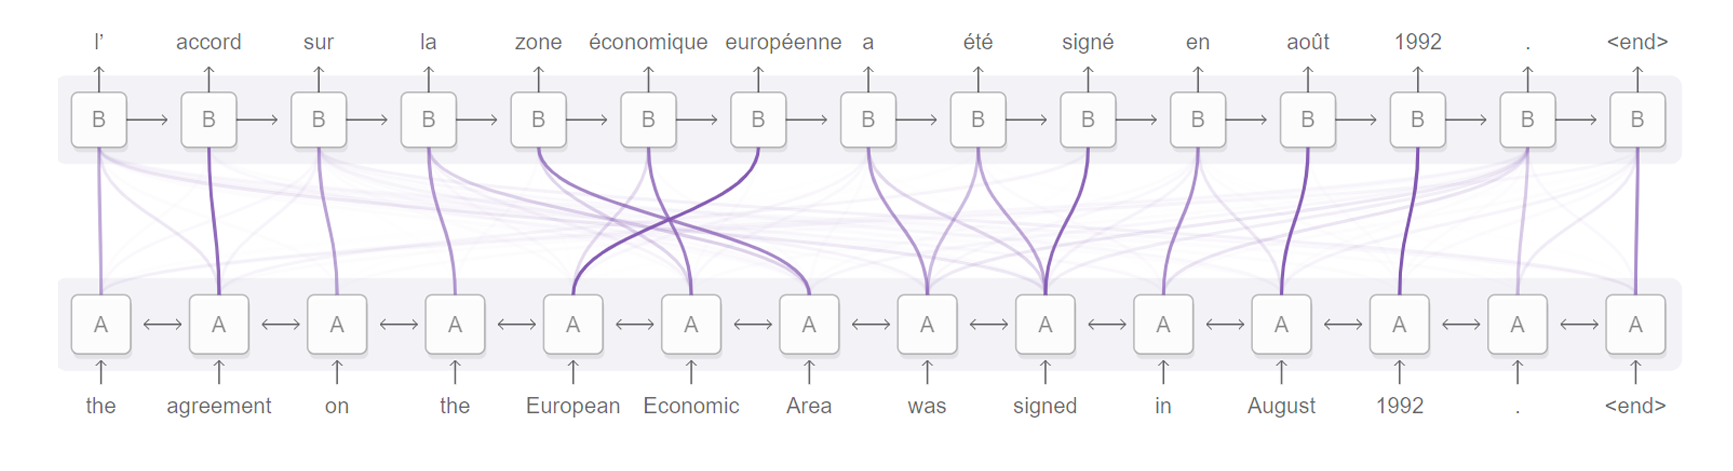
\includegraphics[width=0.8\textwidth]{My-Thesis/Chap1/images/attention_visualization.png}
    \caption{Visualisation de l’attention pour une tâche de traduction : Représentation des poids d’attention montrant les correspondances entre les mots d’une phrase source et sa traduction \cite{lin2017structured}.}
    \label{fig:attention}
\end{figure}

\paragraph{Architectures simplifiées}  
Les architectures simplifiées, comme celles étudiées par \citet{hasani2019compact}, utilisent des réseaux compacts avec un faible nombre de neurones pour faciliter l’analyse des activations. Par exemple, un réseau inspiré du système nerveux d’un ver peut accomplir des tâches complexes tout en restant interprétable grâce à sa simplicité. Dans le contrôle d’accès, de telles architectures pourraient être utilisées pour des décisions simples, comme l’authentification de base, mais elles risquent de manquer de puissance pour des scénarios complexes impliquant de grandes quantités de données.

\paragraph{Avantages et limites}  
Les modèles interprétables offrent une transparence native, idéale pour des applications nécessitant des explications immédiates et compréhensibles. Cependant, leur simplicité peut entraîner une perte de performance par rapport aux modèles plus complexes, ce qui pose un défi dans des contextes comme le contrôle d’accès où la précision est critique.





\mySubSection{Évaluation de l’Explicabilité}{}
L’évaluation de l’explicabilité des modèles d’intelligence artificielle, en particulier des modèles d’apprentissage profond, représente un défi majeur en raison de l’absence de métriques universellement acceptées \cite{jouis2020}. Contrairement aux métriques de performance classiques, telles que la précision ou le rappel, qui sont bien établies, l’explicabilité nécessite des mesures qui tiennent compte à la fois de la fidélité des explications au modèle et de leur compréhensibilité pour les utilisateurs. Cette difficulté est exacerbée par la diversité des contextes d’application et des publics cibles, qui vont des experts techniques aux utilisateurs non initiés.

Les approches pour évaluer l’explicabilité se divisent généralement en deux catégories : les métriques objectives et les métriques subjectives. Les métriques objectives incluent des indicateurs tels que la précision des explications (c’est-à-dire leur capacité à refléter fidèlement les décisions du modèle), le temps de réponse des utilisateurs lorsqu’ils doivent interpréter une explication, ou encore leur capacité à prédire les sorties du modèle à partir des explications fournies \cite{ribeiro2016lime}. Par exemple, dans le cadre de l’évaluation de la méthode des Ancres, des tests avec utilisateurs réels ont montré que des explications sous forme de règles permettent une meilleure compréhension des décisions par rapport à des explications basées sur des poids \cite{ribeiro2016lime}. Les métriques subjectives, quant à elles, se concentrent sur l’acceptabilité des explications et la confiance qu’elles inspirent aux utilisateurs. Ces métriques sont souvent recueillies via des enquêtes ou des retours qualitatifs, mettant en lumière l’importance de la simplicité et de la clarté des explications.


Un aspect crucial de l’évaluation réside dans la prise en compte du contexte et des besoins spécifiques des utilisateurs \cite{dam2018}. Une explication efficace doit être adaptée au niveau d’expertise de son destinataire, qu’il s’agisse d’un administrateur système analysant une décision de contrôle d’accès ou d’un utilisateur final cherchant à comprendre une restriction d’accès. Par exemple, une visualisation comme celle de LIME (voir Figure~\ref{fig:lime}) peut être intuitive pour un utilisateur technique, mais nécessitera une simplification pour un public non expert. De plus, l’évaluation doit refléter l’environnement fonctionnel réel du modèle, afin de garantir que les explications sont pertinentes et utiles dans des scénarios concrets.

\mySubSection{Relevance pour le Contrôle d’Accès}{}
L’application des méthodes d’explicabilité au domaine du contrôle d’accès répond à des besoins critiques en matière de transparence, de conformité réglementaire et de confiance des parties prenantes. Dans des systèmes où les décisions d’accès aux données ou aux traitements sont automatisées, comme dans les infrastructures cloud ou les systèmes IoT, les modèles d’apprentissage profond offrent une grande adaptabilité, mais leur opacité peut compromettre leur adoption. Les réglementations telles que le Règlement Général sur la Protection des Données (RGPD), en particulier son article 22, exigent que les décisions automatisées soient accompagnées d’explications compréhensibles \cite{desmoulin2019}. Cette exigence légale souligne l’importance de méthodes XAI capables de produire des justifications claires et conformes.

Des outils comme LIME ou les Ancres offrent des solutions prometteuses pour le contrôle d’accès. Par exemple, LIME peut être utilisé pour expliquer une décision de refus d’accès en mettant en évidence les facteurs clés, tels que des anomalies dans les métadonnées de connexion (adresse IP, heure d’accès, etc.). Une visualisation comme celle présentée dans la Figure~\ref{fig:lime} pourrait montrer l’importance relative de chaque attribut dans la décision, facilitant ainsi l’audit par un administrateur. De même, les Ancres peuvent générer des règles explicites, comme « Si l’utilisateur se connecte depuis une localisation non autorisée ET à une heure inhabituelle, alors l’accès est refusé », offrant une justification intuitive et vérifiable pour une règle d’accès dynamique \cite{ribeiro2016lime}.

% \begin{figure}[h]
%     \centering
%     \includegraphics[width=0.8\textwidth]{chap1/images/anchor_explanation.png}
%     \caption{Représentation d’une explication avec la méthode des Ancres.}
%     \label{fig:anchor}
% \end{figure}

Cependant, l’intégration de l’explicabilité dans les systèmes de contrôle d’accès soulève des défis spécifiques. Tout d’abord, il est nécessaire de trouver un équilibre entre la performance des modèles, qui repose souvent sur des architectures complexes, et leur explicabilité, qui favorise des explications simples et directes. Ensuite, les explications doivent répondre aux contraintes légales tout en restant accessibles à des utilisateurs variés, allant des régulateurs aux employés \cite{desmoulin2019}. Enfin, les biais potentiels dans les données d’entraînement, qui pourraient conduire à des décisions discriminatoires (par exemple, un refus d’accès basé sur des corrélations démographiques), doivent être détectés et corrigés grâce à des outils d’explicabilité comme SHAP ou LIME.

\mySubSection{Conclusion de la Section}{}
Cette section a exploré les concepts fondamentaux de l’\textit{Explainable Artificial Intelligence} (XAI), en mettant l’accent sur les méthodes d’explicabilité, leur évaluation, et leur application au contrôle d’accès. Les approches comme LIME, les Ancres, et les mécanismes d’attention offrent des moyens concrets pour surmonter l’opacité des modèles d’apprentissage profond, tandis que l’évaluation de l’explicabilité nécessite une combinaison de métriques objectives et subjectives adaptées au contexte. Dans le domaine du contrôle d’accès, l’XAI joue un rôle clé pour garantir la transparence, la conformité aux réglementations, et la confiance des utilisateurs, tout en posant des défis liés à l’équilibre entre performance et compréhensibilité.

L’analyse de ces concepts prépare le terrain pour les sections suivantes du chapitre, qui examineront en détail les systèmes de contrôle d’accès traditionnels et basés sur l’IA, ainsi que les limites des approches existantes en matière d’explicabilité. Ces discussions permettront de mieux contextualiser la nécessité d’une approche XAI spécifiquement adaptée aux besoins du contrôle d’accès.


% %SECTION TRAVAIL COOPERATIF
% %\mySection{Titre}{Titre court}
% \mySection{Le travail coopératif}{}\label{sectionTravailCooperatif}
% Le terme...
% \begin{preuve}
% La preuve
% \end{preuve}

% \mySubSection{L'organisation du travail}{}\label{sectionOrganisationTravail}
% Sur le plan du travail...

% \begin{example}\textit{Le cultivateur et son champ}\\
% Un cultivateur...
% \end{example}

% \mySubSection{Notion de Travail Coopératif Assisté par Ordinateur (CSCW)}{}\label{sectionCSCW}
% La collaboration...

% \mySubSubSection{Les caractéristiques des systèmes de CSCW}{}\label{sectionCaractSystCSCW}
% La mise...

% \myDescription{Système distribué}{Dans un contexte distribué, chaque site possède des copies locales (répliques) des objets partagés et c'est donc sur ces copies que sont portées les contributions locales. Pour obtenir un état global, le système synchronise toutes les répliques. Par conséquent, il est crucial de mettre en place une procédure de contrôle de la concurrence et ce pour assurer la convergence des copies vers un même état.}

% \myDescription{Système non distribué}{Dans...}

% \myDescription{Système synchrone}{Le CSCW est synchrone lorsque les mises à jour apportées par un acteur sur les données partagées sont immédiatement (en un intervalle de temps raisonnable) visibles par l'ensemble des acteurs pouvant avoir accès à ces données. Ces systèmes sont dits temps réel. Les éditeurs collaboratifs temps réel (ou éditeurs WYSIWIS\footnote{What You See Is What I See pouvant être traduit en \textit{ce que vous voyez est ce que je vois}.}) tels que \textit{Etherpad}\footnote{Etherpad est un éditeur collaboratif temps réel disponible à l'adresse \url{http://www.etherpad.org/}.} et \textit{Google Docs}\footnote{L'une des fonctionnalités de Google Docs est la possibilité de réaliser de l'édition temps réel et à plusieurs, \url{https://docs.google.com/}.} en sont de parfaites illustrations.}

% \myDescription{Système asynchrone}{Le...}

% \mySubSubSection{Classification des systèmes de CSCW}{Classification des systèmes de CSCW}
% L'analyse...
% \begin{figure}[h!]
%     \centering
% 		\includegraphics[scale=0.7]{chap1/images/categorizationJoh.png}
%     \caption{Matrice $2\times 2$ de \textit{Johansen} pour la catégorisation des systèmes de CSCW.}
% 	 \label{figCscwToolCateg1}
% \end{figure}





% \chapter{Cadre Théorique}
% \addcontentsline{toc}{chapter}{Cadre Théorique}






% 
\mySection{L’Apprentissage Profond et ses Limites}{}
L’apprentissage profond (\textit{deep learning}, DL) a révolutionné de nombreux domaines grâce à sa capacité à modéliser des relations complexes dans des données volumineuses et non structurées. Cette section vise à établir les bases théoriques du DL, en explorant ses principes fondamentaux, ses applications dans des domaines critiques comme le contrôle d’accès, et les limites inhérentes à son opacité, qui freinent son adoption dans des systèmes où la transparence est essentielle \cite{jouis2020}. L’objectif est de fournir un cadre conceptuel pour comprendre pourquoi l’explicabilité est cruciale pour surmonter ces défis, en particulier dans le contexte de la cybersécurité et de la gestion des accès \cite{zhang2022xai}.

\mySubSection{Introduction à l’Apprentissage Profond}{}
L’apprentissage profond est une sous-discipline de l’apprentissage automatique qui repose sur des réseaux de neurones artificiels organisés en couches multiples, capables de traiter des données complexes sans nécessiter d’ingénierie manuelle des caractéristiques \cite{lecun2015deep}. Apparu comme une approche dominante dans les années 2010, le DL a permis des avancées majeures dans des domaines variés, tels que la reconnaissance d’images, le traitement du langage naturel, et la cybersécurité. Dans le contexte du contrôle d’accès, les modèles de DL sont de plus en plus utilisés pour détecter des anomalies, gérer des permissions dynamiques, et auditer les accès \cite{nobi2022dlbac}. Cette sous-section introduit les concepts clés du DL, met en lumière ses avantages (par exemple, l’extraction automatique de caractéristiques, la robustesse face à des données hétérogènes), et souligne son rôle croissant dans les systèmes critiques où la précision et l’adaptabilité sont primordiales \cite{barredo2020xai}.

\begin{figure}[h]
    \centering
    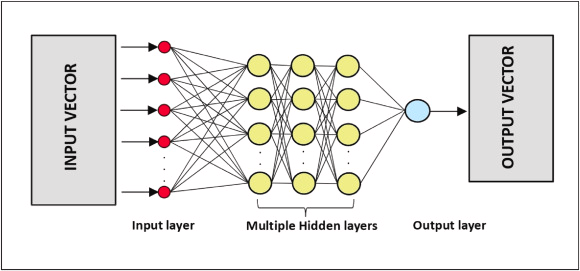
\includegraphics[width=0.8\textwidth]{My-Thesis/Chap1/images/deep_learning_model.png}
    \caption{Représentation schématique d’un réseau de neurones profond, illustrant les couches d’entrée, cachées, et de sortie, ainsi que le flux de données à travers les connexions pondérées. Cette visualisation montre la complexité des architectures de DL, qui contribue à leur puissance mais aussi à leur opacité.}
    \label{fig:dl_overview}
\end{figure}

\mySubSection{Principes Fondamentaux du Deep Learning}{}
\mySubSubSection{Architecture des Réseaux de Neurones}{}
Les réseaux de neurones profonds sont composés de multiples couches de neurones artificiels, interconnectés par des poids appris lors de l’entraînement. Chaque neurone effectue une transformation linéaire suivie d’une fonction d’activation non linéaire (par exemple, ReLU, sigmoïde), permettant au réseau de modéliser des relations complexes \cite{lecun2015deep}. Les architectures courantes incluent les réseaux convolutifs (CNN) pour les données structurées, les réseaux récurrents (RNN) pour les séquences, et les réseaux à attention pour les tâches nécessitant une focalisation sur des éléments spécifiques. Dans le contrôle d’accès, les CNN peuvent analyser des logs formatés, tandis que les RNN sont adaptés à l’analyse des historiques d’accès \cite{karpathy2015visualizing}. Cette sous-section détaille la structure des réseaux, leur modularité, et leur capacité à s’adapter à différents types de données.

\begin{figure}[h]
    \centering
    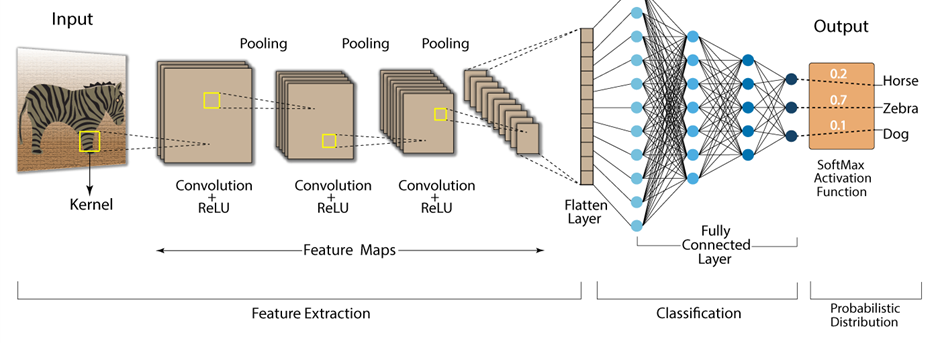
\includegraphics[width=1.0\textwidth]{My-Thesis/Chap1/images/cnn.png}
    \caption{Architecture d’un réseau convolutif (CNN), montrant les couches de convolution, de pooling, et de classification. Cette visualisation illustre comment un CNN extrait des caractéristiques hiérarchiques à partir de données.}
    \label{fig:cnn_architecture}
\end{figure}

\mySubSubSection{Processus d’Entraînement}{}
L’entraînement d’un modèle de DL repose sur la minimisation d’une fonction de perte, qui mesure l’écart entre les prédictions du modèle et les valeurs attendues. Ce processus utilise la rétropropagation du gradient pour ajuster les poids des connexions, souvent via des algorithmes d’optimisation comme la descente de gradient stochastique (SGD) ou Adam \cite{lecun2015deep}. Cette sous-section explique les étapes clés de l’entraînement, les besoins en données volumineuses et étiquetées, et les défis liés à la qualité des données, comme les biais ou les données incomplètes, qui peuvent affecter les performances dans le contrôle d’accès \cite{slack2020fooling}. Elle aborde également l’importance des hyperparamètres (taux d’apprentissage, taille des couches) et des ressources computationnelles nécessaires.

\mySubSubSection{Types de Modèles de Deep Learning}{}
Cette sous-section présente les modèles de DL les plus pertinents pour le contrôle d’accès :
\begin{itemize}
    \item \textbf{Réseaux Convolutifs (CNN)} : Utilisés pour traiter des données structurées, comme les images ou les logs d’accès formatés. Les CNN extraient des motifs spatiaux, utiles pour détecter des anomalies dans les métadonnées d’accès \cite{selvaraju2017gradcam}.
    \item \textbf{Réseaux Récurrents (RNN) et LSTM} : Conçus pour les données séquentielles, comme les historiques d’accès, permettant de modéliser des comportements temporels \cite{karpathy2015visualizing}.
    \item \textbf{Réseaux à Attention} : Ces modèles, comme les transformers, mettent en évidence les attributs critiques (par exemple, localisation ou heure) dans les décisions d’accès \cite{lin2017structured}.
\end{itemize}
Chaque type est illustré par son application potentielle dans le contrôle d’accès, avec un accent sur leur adaptabilité aux environnements dynamiques.

\mySubSection{Applications du Deep Learning dans le Contrôle d’Accès}{}
Le DL offre des solutions puissantes pour moderniser les systèmes de contrôle d’accès, surpassant souvent les approches traditionnelles comme le \textit{Role-Based Access Control} (RBAC) ou l’\textit{Attribute-Based Access Control} (ABAC) \cite{sandhu1996role, hu2013abac}. Cette section explore trois applications clés :
\begin{itemize}
    \item \textbf{Détection d’anomalies} : Les modèles de DL, comme les autoencodeurs ou les RNN, identifient des comportements d’accès inhabituels, tels que des tentatives d’intrusion ou des connexions depuis des localisations non autorisées \cite{nobi2022dlbac}.
    \item \textbf{Gestion dynamique des permissions} : Les réseaux à attention permettent d’adapter les droits d’accès en temps réel en fonction de contextes complexes, comme l’heure, le lieu, ou le type de dispositif \cite{lin2017structured}.
    \item \textbf{Audit des accès} : Les CNN ou LSTM analysent les historiques pour détecter des violations potentielles, offrant une alternative automatisée aux audits manuels \cite{ahmed2021xai}.
\end{itemize}
Des exemples concrets, comme l’utilisation de LSTM pour modéliser des séquences de connexions, sont discutés, avec une comparaison des avantages du DL (flexibilité, précision) et des défis liés à son opacité.


\begin{figure}[h]
    \centering
    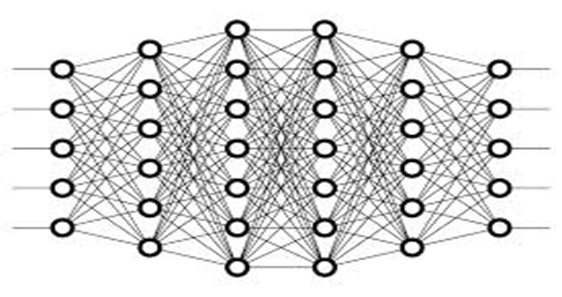
\includegraphics[width=0.8\textwidth]{My-Thesis/Chap1/images/lstm.png}
    \caption{Réseau de neurone complexe.}
    \label{fig:lstm_sequence}
\end{figure}

\mySubSection{Limites du Deep Learning}{}
\mySubSubSection{Opacité des Modèles}{}
Les modèles de DL sont souvent qualifiés de « boîtes noires » en raison de leur complexité architecturale et du grand nombre de paramètres (parfois des millions) \cite{rudin2019stop}. Cette opacité rend difficile l’interprétation des décisions, ce qui pose problème dans le contrôle d’accès, où les administrateurs doivent justifier les refus ou les autorisations d’accès. Cette sous-section explore les raisons techniques de cette opacité, comme la non-linéarité des fonctions d’activation et l’interdépendance des couches, et leurs implications pour la confiance des utilisateurs \cite{jouis2020}.

\mySubSubSection{Biais et Discriminations}{}
Les modèles de DL peuvent hériter ou amplifier des biais présents dans les données d’entraînement, entraînant des décisions discriminatoires, comme le refus d’accès basé sur des corrélations démographiques non pertinentes \cite{slack2020fooling}. Cette partie examine les sources de biais (données déséquilibrées, étiquettes erronées) et leur impact dans le contrôle d’accès, ainsi que les défis pour les détecter et les corriger sans outils d’explicabilité adaptés.

\mySubSubSection{Conformité aux Réglementations}{}
Les réglementations, comme l’article 22 du RGPD, exigent que les décisions automatisées soient accompagnées d’explications compréhensibles \cite{goodman2017gdpr}. Cette sous-section analyse les obstacles à la production d’explications conformes avec les modèles de DL, en raison de leur complexité et de l’absence de méthodes d’explicabilité standardisées. Elle discute des implications pour les systèmes de contrôle d’accès, où la conformité est cruciale \cite{desmoulin2019}.

% \begin{figure}[h]
%     \centering
%     \includegraphics[width=0.8\textwidth]{bias_visualization.png}
%     \caption{Représentation des biais dans un modèle de DL pour le contrôle d’accès, montrant comment des corrélations non pertinentes (par exemple, démographiques) peuvent influencer une décision de refus d’accès. Cette visualisation met en évidence la nécessité d’outils d’explicabilité pour détecter ces biais.}
%     \label{fig:bias_visualization}
% \end{figure}

\mySubSection{Nécessité de l’Explicabilité}{}
Face aux limites du DL, l’\textit{Explainable Artificial Intelligence} (XAI) émerge comme une solution pour rendre les modèles plus transparents et conformes. Cette section introduit les principales méthodes d’explicabilité, telles que LIME (approximation linéaire locale), SHAP (valeurs de Shapley), et les mécanismes d’attention, qui permettent de justifier les décisions des modèles \cite{ribeiro2016lime, lundberg2017shap, lin2017structured}. Elle souligne leur pertinence pour le contrôle d’accès, où les explications doivent être à la fois précises, compréhensibles, et conformes aux exigences légales \cite{barredo2020xai}. Une discussion sur l’équilibre entre performance et explicabilité conclut cette partie.

\mySubSection{Conclusion de la Section}{}
Cette section a exploré les principes fondamentaux, les applications, et les limites de l’apprentissage profond, en mettant l’accent sur son rôle dans le contrôle d’accès. Si le DL offre une puissance et une flexibilité inégalées, son opacité, ses biais potentiels, et les défis de conformité réglementaire nécessitent des approches d’explicabilité robustes. Ces concepts préparent le terrain pour les sections suivantes, qui analyseront les méthodes d’explicabilité et les systèmes de contrôle d’accès traditionnels et basés sur l’IA.

% 

\mySection{L'Explainable Artificial Intelligence (XAI)}{}\label{sectionXAICadre}

\mySubSection{Introduction à l’XAI}{}\label{xaiIntro}
L'\textit{Explainable Artificial Intelligence} (XAI), ou intelligence artificielle explicable, émerge comme une discipline clé visant à rendre les modèles d'intelligence artificielle compréhensibles pour les humains. Cette nécessité découle de l'opacité inhérente à de nombreux modèles, notamment ceux basés sur l'apprentissage profond, souvent qualifiés de "boîtes noires" en raison de la difficulté à interpréter leurs processus décisionnels \cite{jouis2020}. L'explicabilité est particulièrement cruciale dans des contextes où la transparence et la confiance sont essentielles, comme le contrôle d'accès aux données et aux traitements. Dans ce domaine, une décision non justifiée peut entraîner des conséquences graves, telles que des violations de sécurité ou des atteintes à la vie privée. L'essor récent de l'XAI, motivé par ces limites, s'inscrit dans une volonté de répondre aux attentes des utilisateurs et aux exigences réglementaires, tout en maintenant les performances des modèles \cite{jouis2020}.

\mySubSection{Définitions et Objectifs de l’XAI}{}
L'explicabilité peut être définie comme la capacité d'un modèle à fournir des explications compréhensibles par un humain, que ce soit en décrivant son fonctionnement global ou en justifiant une décision spécifique \cite{miller2019explanation}. Cette transparence vise à permettre aux utilisateurs, qu'ils soient experts ou non, de comprendre les raisons sous-jacentes aux prédictions ou aux décisions automatisées. Les objectifs principaux de l'XAI incluent l'amélioration de la confiance des utilisateurs envers les systèmes intelligents, la facilitation de l'audit des modèles pour détecter d'éventuels biais ou erreurs, et la conformité aux exigences légales et éthiques, telles que celles imposées par le Règlement Général sur la Protection des Données (RGPD) \cite{gilpin2018explaining}. Une distinction fondamentale est faite entre l'explicabilité globale, qui cherche à comprendre le comportement général du modèle, et l'explicabilité locale, qui se concentre sur l'explication d'une décision particulière pour une instance donnée \cite{ribeiro2016lime}.



\mySubSection{Taxonomie des Méthodes d’Explicabilité}{}
Les méthodes d'explicabilité des modèles d'apprentissage profond peuvent être classées en trois grandes catégories en fonction de leur niveau de transparence vis-à-vis de la structure interne du modèle \cite{jouis2020, guidotti2018}. Cette taxonomie, illustrée dans la littérature par des approches variées, permet de structurer les techniques selon qu'elles traitent le modèle comme une boîte noire, une boîte grise ou une boîte blanche. Chaque catégorie répond à des contraintes techniques et à des besoins spécifiques des utilisateurs, qu’il s’agisse de simplicité, de fidélité au modèle ou de compréhensibilité. La figure~\ref{fig:taxonomie_xai} illustre schématiquement ces trois approches en fonction de leur dépendance à l'architecture du modèle et de leur niveau d'interprétabilité.

\begin{figure}[h]
    \centering
    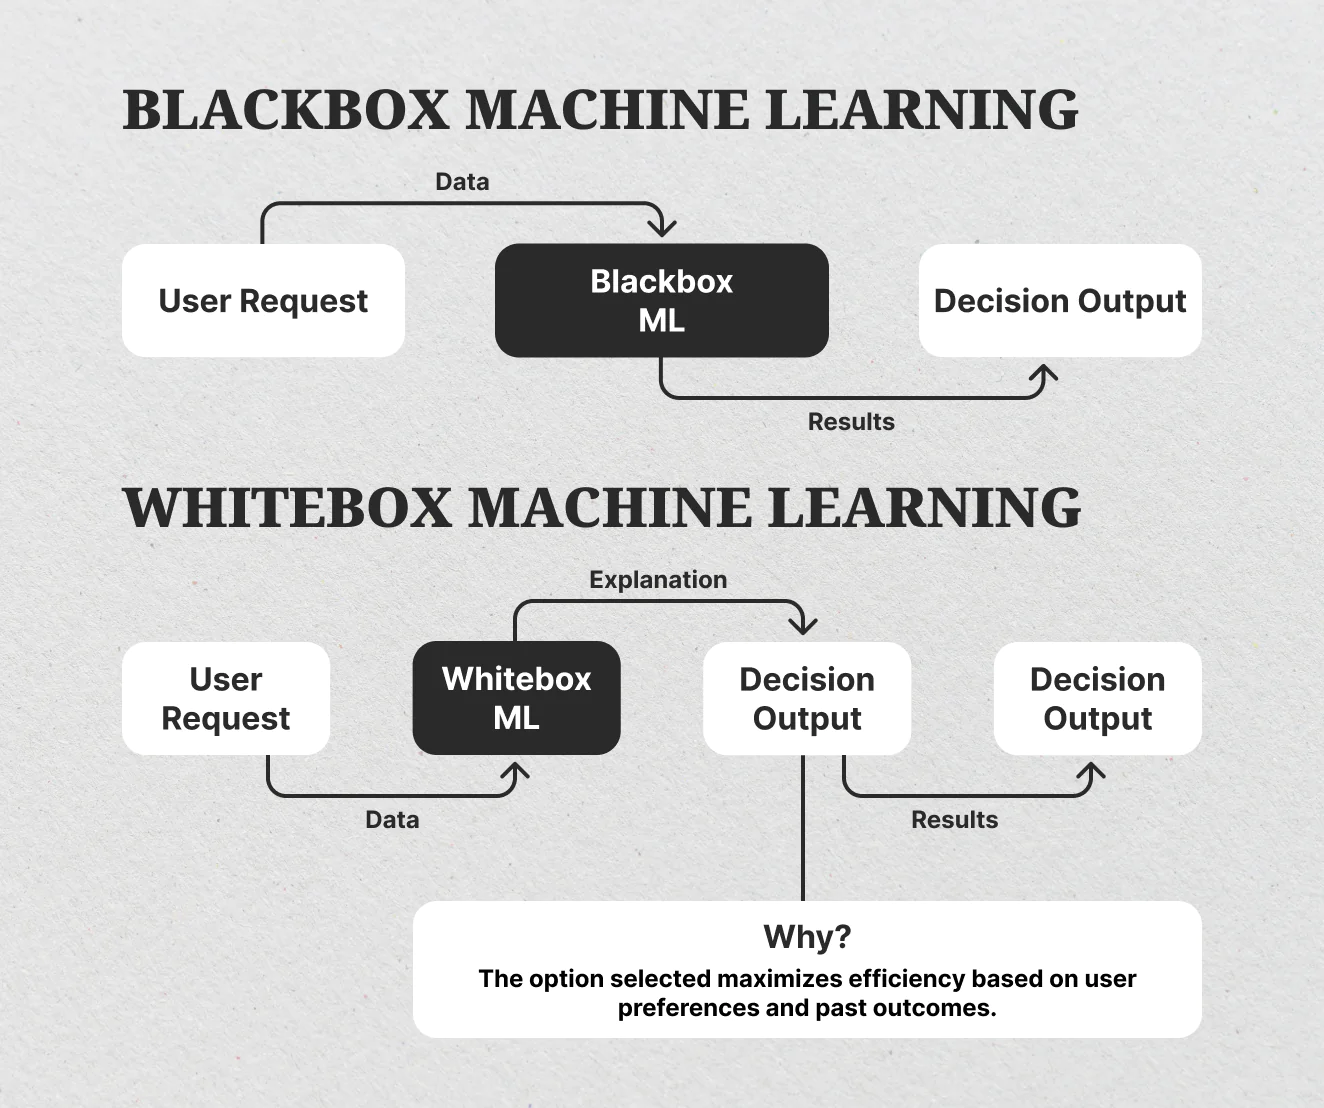
\includegraphics[width=0.8\textwidth]{My-Thesis/Chap1/images/taxonomy.png}
    \caption{Taxonomie des méthodes d'explicabilité : boîte noire (indépendante du modèle), et boîte blanche (modèle interprétable). L'axe vertical représente le niveau d'interprétabilité}
    \label{fig:taxonomie_xai}
\end{figure}

\begin{itemize}
    \item \textbf{Approches indépendantes du modèle (boîte noire)} : Ces méthodes analysent les entrées et sorties du modèle sans accéder à sa structure interne. Elles sont flexibles, car applicables à tout type de modèle, mais reposent souvent sur des corrélations plutôt que sur des causalités. Par exemple, des outils comme LIME ou SHAP quantifient l'impact des variables d'entrée sur les prédictions \cite{guidotti2018}. Elles sont particulièrement adaptées lorsque la priorité est de fournir des explications rapides et générales, sans nécessiter une expertise approfondie de l'architecture sous-jacente. Cependant, leur fidélité peut être limitée, car elles ne capturent pas toujours les mécanismes précis du modèle.
    % \begin{figure}
    %     \centering
    %     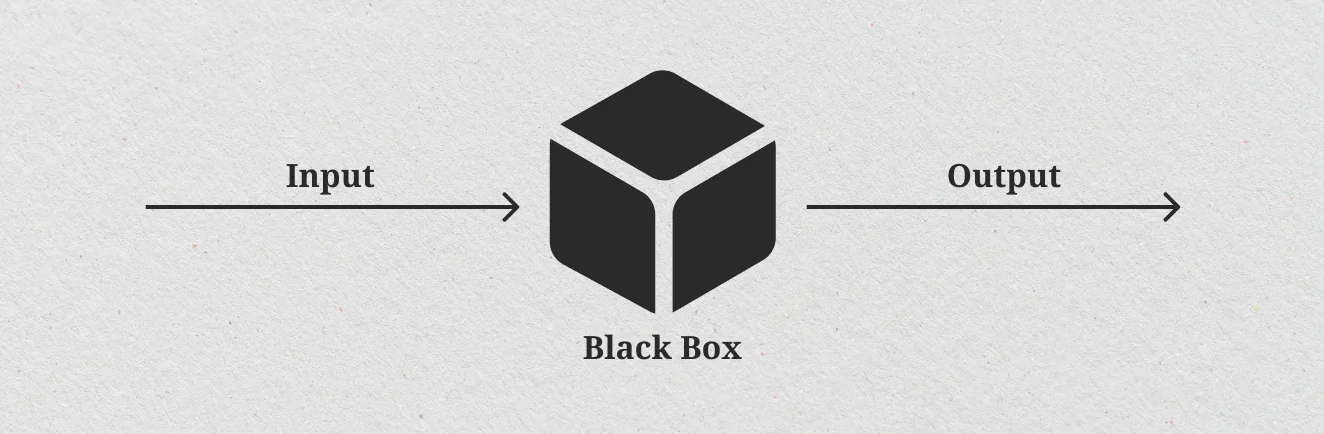
\includegraphics[width=0.6\linewidth]{chap1//images/blackbox_ai.png}
    %     \caption{modele boite noire}
    %     \label{fig:enter-label}
    % \end{figure}

    \item \textbf{Approches dépendantes du modèle (boîte grise)} : Ces techniques exploitent les paramètres internes du modèle, comme les poids des neurones ou les activations des couches, pour générer des explications. Elles offrent une meilleure fidélité, car elles reflètent directement le fonctionnement du modèle, mais sont contraintes par l'architecture spécifique (par exemple, CNN ou LSTM) \cite{jouis2020}. Des méthodes comme Grad-CAM, qui produit des cartes de chaleur pour les réseaux convolutifs, permettent de visualiser les régions influentes d’une entrée \cite{selvaraju2017gradcam}. Ces approches conviennent aux scénarios où une compréhension fine du modèle est nécessaire, mais elles exigent des compétences techniques pour interpréter les résultats.

    \item \textbf{Modèles interprétables (boîte blanche)} : Ces approches intègrent l'explicabilité dès la conception du modèle, en utilisant des architectures intrinsèquement transparentes, comme les mécanismes d'attention ou des réseaux simplifiés \cite{jouis2020}. Elles garantissent une compréhensibilité élevée, car les explications sont directement dérivées des paramètres du modèle, mais peuvent sacrifier une partie des performances par rapport aux modèles complexes. Elles sont idéales pour les applications où la transparence est une priorité absolue, comme dans les systèmes critiques soumis à des réglementations strictes.

\end{itemize}

Chaque catégorie présente des avantages et des limites, qui dépendent des contraintes du projet et des attentes des utilisateurs. Par exemple, dans le cadre du contrôle d'accès, les approches indépendantes du modèle peuvent être privilégiées pour leur flexibilité, tandis que les modèles interprétables sont mieux adaptés pour répondre aux exigences légales de transparence, comme celles imposées par le RGPD \cite{guidotti2018}. Le choix d’une méthode doit donc équilibrer la fidélité des explications, leur compréhensibilité et les ressources disponibles pour leur mise en œuvre.





\mySubSection{Méthodes Spécifiques d’Explicabilité}{}

Cette section détaille les principales méthodes d'explicabilité utilisées pour rendre les modèles d'apprentissage profond plus transparents, en se concentrant sur leur application potentielle au contrôle d'accès. Ces approches sont classées en trois catégories selon leur dépendance à l'architecture du modèle : approches indépendantes du modèle, approches dépendantes du modèle, et modèles interprétables. Chaque méthode est illustrée, lorsque pertinent, par des visualisations issues de la littérature.

\mySubSubSection{Approches indépendantes du modèle}{}

Les approches indépendantes du modèle, souvent qualifiées d'agnostiques, permettent d'expliquer les prédictions sans nécessiter une connaissance approfondie de la structure interne du modèle. Elles se basent principalement sur l'analyse des relations entre les entrées et les sorties, offrant ainsi une grande flexibilité d'application.

\paragraph{LIME (Local Interpretable Model-agnostic Explanations)}  
L'outil LIME, proposé par \cite{ribeiro2016lime}, génère des explications locales en approximant le comportement d'un modèle complexe autour d'une instance spécifique à l'aide d'un modèle linéaire simple. Pour une prédiction donnée, LIME identifie les variables d'entrée ayant le plus d'impact, comme les mots dans un texte ou les pixels dans une image, et quantifie leur influence positive ou négative sur la décision. Cette méthode est particulièrement utile pour expliquer des décisions dans des contextes comme le contrôle d'accès, où il peut être nécessaire de justifier pourquoi un accès a été refusé en mettant en évidence des facteurs clés (par exemple, une tentative d'accès à une heure inhabituelle).  

\begin{figure}[h]
    \centering
    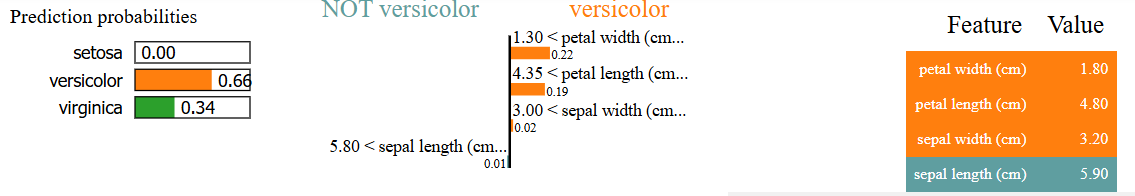
\includegraphics[width=0.8\textwidth]{My-Thesis/Chap1/images/lime_explanation.png}
    \caption{LIME : Visualisation de l’importance des mots dans une prédiction textuelle, où chaque mot est associé à un poids reflétant son influence sur la classe prédite \citep{ribeiro2016why}.}
    \label{fig:lime}
\end{figure}

\paragraph{Ancres}  
Les Ancres, une amélioration de LIME proposée par \citet{ribeiro2018anchors}, fournissent des explications sous forme de règles logiques définissant le contexte dans lequel une prédiction est valide. Par exemple, pour une décision de contrôle d'accès, une ancre pourrait être : "Si l’utilisateur tente d’accéder depuis un emplacement non autorisé et à une heure inhabituelle, alors l’accès est refusé." Ces règles sont construites pour maximiser la précision (fidélité au modèle) et la couverture (généralisation à d’autres instances similaires). Cette approche est particulièrement adaptée pour des systèmes nécessitant des justifications claires et compréhensibles par des utilisateurs non techniques.

\begin{figure}[h]
    \centering
    \includegraphics[width=0.8\textwidth]{My-Thesis/Chap1/images/anchor_explanation.png}
    \caption{Anchor : Visualisation des parties importantes d’une entrée (par exemple, mots ou régions d’image) définissant une règle d’explication pour une prédiction spécifique \citep{ribeiro2018anchors}.}
    \label{fig:anchor}
\end{figure}

\paragraph{Valeurs de Shapley et SHAP}  
Inspirées de la théorie des jeux, les valeurs de Shapley quantifient la contribution de chaque variable d’entrée à une prédiction \citep{lundberg2017shap}. Le module SHAP (\textit{Shapley Additive Explanations}) optimise ce calcul pour le rendre applicable à des modèles complexes, en fournissant une mesure de l’importance des variables sous forme de scores additifs. Par exemple, dans le cadre du contrôle d’accès, SHAP pourrait révéler qu’une tentative d’accès a été refusée principalement en raison de l’historique des connexions de l’utilisateur. Cependant, cette méthode peut être difficile à interpréter pour des utilisateurs non experts en raison de la complexité des calculs et de la nécessité d’un post-traitement pour simplifier les résultats.

\paragraph{Limites}  
Les approches indépendantes du modèle, bien que flexibles, présentent des limites. Elles mettent en évidence des corrélations entre entrées et sorties, mais ne garantissent pas une compréhension causale des décisions. De plus, leur complexité peut rendre les explications difficiles à assimiler pour des utilisateurs sans expertise technique, en particulier dans des domaines comme le contrôle d’accès où les explications doivent être conformes aux réglementations.

\mySubSubSection{Approches dépendantes du modèle}{}

Les approches dépendantes du modèle exploitent la structure interne du modèle pour générer des explications plus fidèles à son fonctionnement. Elles nécessitent une connaissance de l’architecture, ce qui limite leur applicabilité mais améliore leur précision.

\paragraph{Grad-CAM}  
La méthode Grad-CAM (\textit{Gradient-weighted Class Activation Mapping}), proposée par \cite{selvaraju2017gradcam}, génère des cartes de chaleur pour visualiser les régions d’une entrée (généralement une image) influençant une prédiction dans un réseau convolutif (CNN). Bien que principalement utilisée pour l’analyse d’images, cette méthode pourrait être adaptée au contrôle d’accès pour des données visuelles, comme des captures d’écran de tentatives d’accès frauduleuses, en mettant en évidence les zones critiques de l’image. La fidélité de Grad-CAM à la décision du modèle en fait un outil puissant, mais son application est restreinte aux architectures convolutives.


\begin{figure}[h]
    \centering
    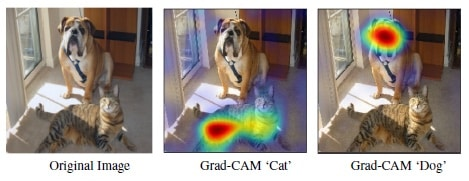
\includegraphics[width=0.8\textwidth]{My-Thesis/Chap1/images/gradcam_visualization.png}
    \caption{Visualisation d'une explication Grad-CAM.}
    \label{fig:gradcam}
\end{figure}

dans la figure \ref{fig:gradcam}, la Carte de chaleur met en évidence les régions d’une image influençant la classification dans un réseau convolutif, comme les zones pertinentes pour identifier une classe spécifique, l'un pour les chiens et l'autre pour les chats. \citep{GradCAMImage}

\paragraph{Analyse des LSTM}  
Les réseaux Long Short-Term Memory (LSTM) sont largement utilisés pour l’analyse de séquences, comme les logs d’accès dans un système de contrôle. \citet{karpathy2015visualizing} proposent d’étudier les activations des cellules LSTM pour comprendre les motifs détectés, comme la reconnaissance de motifs spécifiques dans un texte (par exemple, des guillemets indiquant une citation). Dans le contexte du contrôle d’accès, cette méthode pourrait révéler pourquoi un modèle a identifié une séquence d’actions comme suspecte. Cependant, l’analyse des activations est complexe et nécessite une exploration approfondie, ce qui peut limiter son accessibilité.


\begin{figure}[h]
    \centering
    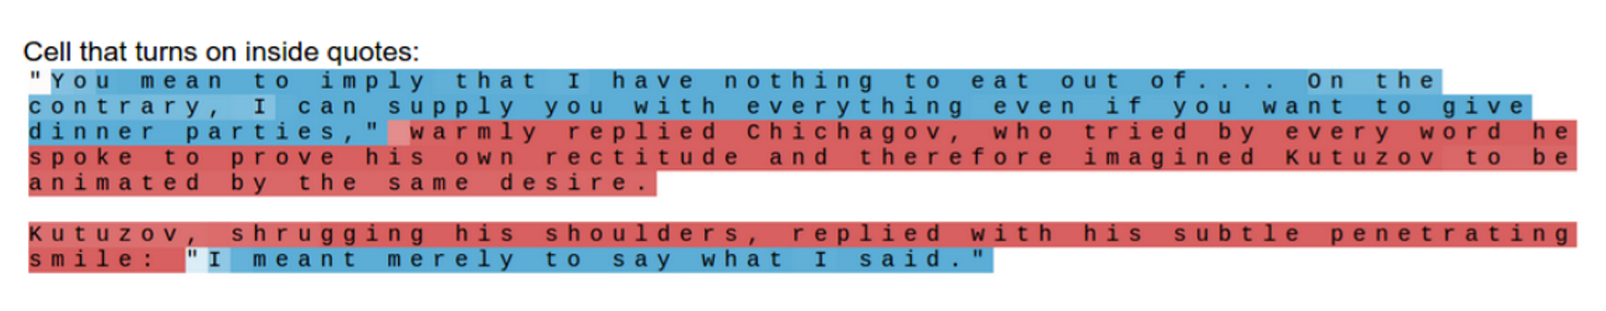
\includegraphics[width=0.8\textwidth]{My-Thesis/Chap1/images/lstm_activation.png}
    \caption{Activation d’une cellule en fonction des guillemets dans le texte : Visualisation des activations d’une cellule LSTM détectant des motifs textuels spécifiques, comme les guillemets \citep{karpathy2015visualizing}.}
    \label{fig:lstm}
\end{figure}

\paragraph{Avantages et inconvénients}  
Les approches dépendantes du modèle offrent une grande fidélité, car elles s’appuient directement sur les mécanismes internes du modèle. Elles sont particulièrement utiles pour des experts souhaitant auditer un système de contrôle d’accès. Cependant, leur dépendance à l’architecture limite leur généralisation, et leur complexité peut poser des défis pour des explications destinées à des utilisateurs non techniques.

\mySubSubSection{Modèles interprétables}{}

Les modèles interprétables, ou boîtes blanches, sont conçus pour être transparents par leur architecture, réduisant ainsi le besoin d’analyses post-entraînement.

\paragraph{Mécanismes d’attention}  
Les mécanismes d’attention, décrits par \cite{lin2017structured}, permettent de visualiser les poids attribués aux différentes parties d’une entrée, comme les mots dans une phrase. Dans une tâche de traduction, par exemple, les poids d’attention mettent en évidence les correspondances entre mots source et cible. Appliqués au contrôle d’accès, ces mécanismes pourraient identifier les éléments clés d’une requête d’accès (par exemple, un identifiant utilisateur ou une adresse IP) influençant la décision. Cette approche est intuitive et ne nécessite pas de calculs supplémentaires après l’entraînement, mais elle est spécifique aux modèles intégrant une couche d’attention.



\begin{figure}[h]
    \centering
    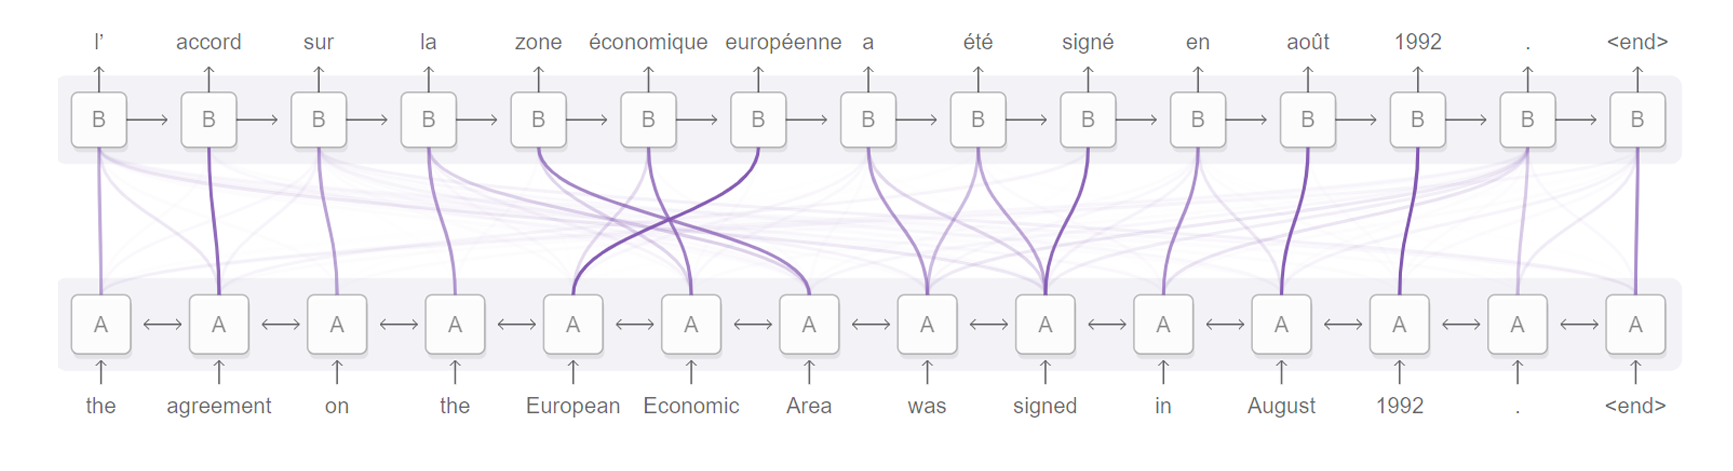
\includegraphics[width=0.8\textwidth]{My-Thesis/Chap1/images/attention_visualization.png}
    \caption{Visualisation de l’attention pour une tâche de traduction : Représentation des poids d’attention montrant les correspondances entre les mots d’une phrase source et sa traduction \cite{lin2017structured}.}
    \label{fig:attention}
\end{figure}

\paragraph{Architectures simplifiées}  
Les architectures simplifiées, comme celles étudiées par \citet{hasani2019compact}, utilisent des réseaux compacts avec un faible nombre de neurones pour faciliter l’analyse des activations. Par exemple, un réseau inspiré du système nerveux d’un ver peut accomplir des tâches complexes tout en restant interprétable grâce à sa simplicité. Dans le contrôle d’accès, de telles architectures pourraient être utilisées pour des décisions simples, comme l’authentification de base, mais elles risquent de manquer de puissance pour des scénarios complexes impliquant de grandes quantités de données.

\paragraph{Avantages et limites}  
Les modèles interprétables offrent une transparence native, idéale pour des applications nécessitant des explications immédiates et compréhensibles. Cependant, leur simplicité peut entraîner une perte de performance par rapport aux modèles plus complexes, ce qui pose un défi dans des contextes comme le contrôle d’accès où la précision est critique.





\mySubSection{Évaluation de l’Explicabilité}{}
L’évaluation de l’explicabilité des modèles d’intelligence artificielle, en particulier des modèles d’apprentissage profond, représente un défi majeur en raison de l’absence de métriques universellement acceptées \cite{jouis2020}. Contrairement aux métriques de performance classiques, telles que la précision ou le rappel, qui sont bien établies, l’explicabilité nécessite des mesures qui tiennent compte à la fois de la fidélité des explications au modèle et de leur compréhensibilité pour les utilisateurs. Cette difficulté est exacerbée par la diversité des contextes d’application et des publics cibles, qui vont des experts techniques aux utilisateurs non initiés.

Les approches pour évaluer l’explicabilité se divisent généralement en deux catégories : les métriques objectives et les métriques subjectives. Les métriques objectives incluent des indicateurs tels que la précision des explications (c’est-à-dire leur capacité à refléter fidèlement les décisions du modèle), le temps de réponse des utilisateurs lorsqu’ils doivent interpréter une explication, ou encore leur capacité à prédire les sorties du modèle à partir des explications fournies \cite{ribeiro2016lime}. Par exemple, dans le cadre de l’évaluation de la méthode des Ancres, des tests avec utilisateurs réels ont montré que des explications sous forme de règles permettent une meilleure compréhension des décisions par rapport à des explications basées sur des poids \cite{ribeiro2016lime}. Les métriques subjectives, quant à elles, se concentrent sur l’acceptabilité des explications et la confiance qu’elles inspirent aux utilisateurs. Ces métriques sont souvent recueillies via des enquêtes ou des retours qualitatifs, mettant en lumière l’importance de la simplicité et de la clarté des explications.


Un aspect crucial de l’évaluation réside dans la prise en compte du contexte et des besoins spécifiques des utilisateurs \cite{dam2018}. Une explication efficace doit être adaptée au niveau d’expertise de son destinataire, qu’il s’agisse d’un administrateur système analysant une décision de contrôle d’accès ou d’un utilisateur final cherchant à comprendre une restriction d’accès. Par exemple, une visualisation comme celle de LIME (voir Figure~\ref{fig:lime}) peut être intuitive pour un utilisateur technique, mais nécessitera une simplification pour un public non expert. De plus, l’évaluation doit refléter l’environnement fonctionnel réel du modèle, afin de garantir que les explications sont pertinentes et utiles dans des scénarios concrets.

\mySubSection{Relevance pour le Contrôle d’Accès}{}
L’application des méthodes d’explicabilité au domaine du contrôle d’accès répond à des besoins critiques en matière de transparence, de conformité réglementaire et de confiance des parties prenantes. Dans des systèmes où les décisions d’accès aux données ou aux traitements sont automatisées, comme dans les infrastructures cloud ou les systèmes IoT, les modèles d’apprentissage profond offrent une grande adaptabilité, mais leur opacité peut compromettre leur adoption. Les réglementations telles que le Règlement Général sur la Protection des Données (RGPD), en particulier son article 22, exigent que les décisions automatisées soient accompagnées d’explications compréhensibles \cite{desmoulin2019}. Cette exigence légale souligne l’importance de méthodes XAI capables de produire des justifications claires et conformes.

Des outils comme LIME ou les Ancres offrent des solutions prometteuses pour le contrôle d’accès. Par exemple, LIME peut être utilisé pour expliquer une décision de refus d’accès en mettant en évidence les facteurs clés, tels que des anomalies dans les métadonnées de connexion (adresse IP, heure d’accès, etc.). Une visualisation comme celle présentée dans la Figure~\ref{fig:lime} pourrait montrer l’importance relative de chaque attribut dans la décision, facilitant ainsi l’audit par un administrateur. De même, les Ancres peuvent générer des règles explicites, comme « Si l’utilisateur se connecte depuis une localisation non autorisée ET à une heure inhabituelle, alors l’accès est refusé », offrant une justification intuitive et vérifiable pour une règle d’accès dynamique \cite{ribeiro2016lime}.

% \begin{figure}[h]
%     \centering
%     \includegraphics[width=0.8\textwidth]{chap1/images/anchor_explanation.png}
%     \caption{Représentation d’une explication avec la méthode des Ancres.}
%     \label{fig:anchor}
% \end{figure}

Cependant, l’intégration de l’explicabilité dans les systèmes de contrôle d’accès soulève des défis spécifiques. Tout d’abord, il est nécessaire de trouver un équilibre entre la performance des modèles, qui repose souvent sur des architectures complexes, et leur explicabilité, qui favorise des explications simples et directes. Ensuite, les explications doivent répondre aux contraintes légales tout en restant accessibles à des utilisateurs variés, allant des régulateurs aux employés \cite{desmoulin2019}. Enfin, les biais potentiels dans les données d’entraînement, qui pourraient conduire à des décisions discriminatoires (par exemple, un refus d’accès basé sur des corrélations démographiques), doivent être détectés et corrigés grâce à des outils d’explicabilité comme SHAP ou LIME.

\mySubSection{Conclusion de la Section}{}
Cette section a exploré les concepts fondamentaux de l’\textit{Explainable Artificial Intelligence} (XAI), en mettant l’accent sur les méthodes d’explicabilité, leur évaluation, et leur application au contrôle d’accès. Les approches comme LIME, les Ancres, et les mécanismes d’attention offrent des moyens concrets pour surmonter l’opacité des modèles d’apprentissage profond, tandis que l’évaluation de l’explicabilité nécessite une combinaison de métriques objectives et subjectives adaptées au contexte. Dans le domaine du contrôle d’accès, l’XAI joue un rôle clé pour garantir la transparence, la conformité aux réglementations, et la confiance des utilisateurs, tout en posant des défis liés à l’équilibre entre performance et compréhensibilité.

L’analyse de ces concepts prépare le terrain pour les sections suivantes du chapitre, qui examineront en détail les systèmes de contrôle d’accès traditionnels et basés sur l’IA, ainsi que les limites des approches existantes en matière d’explicabilité. Ces discussions permettront de mieux contextualiser la nécessité d’une approche XAI spécifiquement adaptée aux besoins du contrôle d’accès.



















% \mySection{Conclusion du Chapitre}\label{sectionconclussionChap1}
% Ce chapitre conclut en résumant les concepts clés abordés, notamment les principes de l'apprentissage profond, les méthodes d'explicabilité, les systèmes de contrôle d'accès, et les exigences des environnements critiques. Il souligne l'importance de combler le fossé entre performance et transparence pour permettre une adoption sûre et efficace des modèles d'apprentissage profond dans le contrôle d'accès. Enfin, il prépare le terrain pour le chapitre suivant, qui examinera les approches existantes et leurs limites.



\mySection{Synthèse}{}\label{sectionSyntheseChap1}
Ce chapitre conclut en résumant les concepts clés abordés, notamment les principes de l'apprentissage profond, les méthodes d'explicabilité, les systèmes de contrôle d'accès, et les exigences des environnements critiques. Il souligne l'importance de combler le fossé entre performance et transparence pour permettre une adoption sûre et efficace des modèles d'apprentissage profond dans le contrôle d'accès. Enfin, il prépare le terrain pour le chapitre suivant, qui examinera les approches existantes et leurs limites.


	\myChapter{État de l'art}{}\label{chapEditionStructure}

% \begin{table}
% 	\caption{Un tableau}
% 	\begin{flushleft}
% 	\begin{tabular}[t]{lcp{5.3cm}l}
% 	$\langle A,w_{1} \rangle$ & $\longrightarrow$ & $(P_{1}, [\langle C,u \rangle, \langle B,v \rangle])$ & si $w_{1}=u[v]$ \\
	
% 	\end{tabular}
% 	\begin{tabular}[t]{lcp{5.3cm}l}
	
% 	$\langle A,w_{2} \rangle$ & $\longrightarrow$ & $(P_{1}, [\langle C,u \rangle, \langle B,w_{11} \rangle])$ & si $w_{2}=uw_{11}$ avec $w_{11}=[_{\omega}\, ]_{\omega}$ \\
	
% 	\end{tabular}
% 	\begin{tabular}[t]{lcp{5.3cm}l}
	
% 	$\langle A,w_{3} \rangle$ & $\longrightarrow$ & $(P_{2}, [\,])$ & si $w_{3}=\epsilon$\\
	
% 	\end{tabular}
% 	\begin{tabular}[t]{lcp{5.3cm}l}
	
% 	$\langle A,w_{4} \rangle$ & $\longrightarrow$ & $(A_{\omega}, [\,])$ & si $w_{4}=(_{\omega}\, )_{\omega}$\\
	
% 	\end{tabular}
% 	\begin{tabular}[t]{lcp{5.3cm}l}
	
% 	$\langle B,w_{5} \rangle$ & $\longrightarrow$ & $(P_{3}, [\langle C,u \rangle, \langle A,v \rangle])$ & si $w_{5}=u(v)$ \\
	
% 	\end{tabular}
% 	\begin{tabular}[t]{lcp{5.3cm}l}
	
% 	$\langle B,w_{6} \rangle$ & $\longrightarrow$ & $(P_{3}, [\langle C,u \rangle, \langle A,w_{4} \rangle])$ & si $w_{6}=uw_{4}$ \\
	
% 	\end{tabular}
% 	\begin{tabular}[t]{lcp{5.3cm}l}
	
% 	$\langle B,w_{7} \rangle$ & $\longrightarrow$ & $(P_{4}, [\langle B,u \rangle, \langle B,v \rangle])$ & si $w_{7}=[u][v]$\\
	
% 	\end{tabular}
% 	\begin{tabular}[t]{lcp{5.3cm}l}
	
% 	$\langle B,w_{8} \rangle$ & $\longrightarrow$ & $(P_{4}, [\langle B,w_{11} \rangle, \langle B,v \rangle])$ & si $w_{8}=w_{11}[v]$\\
	
% 	\end{tabular}
% 	\begin{tabular}[t]{lcp{5.3cm}l}
	
% 	$\langle B,w_{9} \rangle$ & $\longrightarrow$ & $(P_{4}, [\langle B,u \rangle, \langle B,w_{11} \rangle])$ & si $w_{9}=[u]w_{11}$\\
	
% 	\end{tabular}
% 	\begin{tabular}[t]{lcp{5.3cm}l}
	
% 	$\langle B,w_{10} \rangle$ & $\longrightarrow$ & $(P_{4}, [\langle B,w_{11} \rangle, \langle B,w_{11} \rangle])$ & si $w_{10}=w_{11}w_{11}$\\
	
% 	\end{tabular}
% 	\begin{tabular}[t]{lcp{5.3cm}l}
	
% 	$\langle B,w_{11} \rangle$ & $\longrightarrow$ & $(B_{\omega}, [\,])$ & si $w_{11}=[_{\omega}\, ]_{\omega}$\\
	
% 	\end{tabular}
% 	\begin{tabular}[t]{lcp{5.3cm}l}
	
% 	$\langle C,w_{12} \rangle$ & $\longrightarrow$ & $(P_{5}, [\langle A,u \rangle, \langle C,v \rangle])$ & si $w_{12}=(u)v$ \\
	
% 	\end{tabular}
% 	\begin{tabular}[t]{lcp{5.3cm}l}
	
% 	$\langle C,w_{13} \rangle$ & $\longrightarrow$ & $(P_{5}, [\langle A,w_{4} \rangle, \langle C,v \rangle])$ & si $w_{13}=w_{4}v$ \\
	
% 	\end{tabular}
% 	\begin{tabular}[t]{lcp{5.3cm}l}
	
% 	$\langle C,w_{14} \rangle$ & $\longrightarrow$ & $(P_{6}, [\langle C,u \rangle, \langle C,v \rangle])$ & si $w_{14}=uv\neq\epsilon$\\
	
% 	\end{tabular}
% 	\begin{tabular}[t]{lcp{5.3cm}l}
	
% 	$\langle C,w_{15} \rangle$ & $\longrightarrow$ & $(C_\omega,[\,])$ & si $w_{15}=\epsilon$\\
	
% 	\end{tabular}
% 	\end{flushleft}
% \end{table}

	\part{Notre Travail}
	


\myChapter{Proposition méthodologique}{}\label{chapFusionConsens}

	

\myChapter{Expérimentations}{}\label{chapTinyCE}

	
	%Ainsi de suite
	
	%\myChapterStar{Titre}{Titre court}{Ajouter à la table des matières? (false|true|chapter|section|subsection|subsubsection -chapter par défaut-)}
\myChapterStar{Conclusion générale}{}{true}
\myMiniToc{}{Contents}

Le bilan...

%\mySectionStar{Titre}{Titre court}{Ajouter à la table des matières? (false|true|chapter|section|subsection|subsubsection -section par défaut-)}
\mySectionStar{La problématique étudiée et les choix méthodologiques}{}{true}
Nous... 

\mySectionStar{Analyse critique des résultats obtenus}{}{true}
Sachant...

\mySectionStar{Quelques perspectives}{}{true}
Ce travail...



\myCleanStarChapterEnd

	
	%************ Bibliographie ***************
	% La charte de l'école doctorale recommande un style dans lequel les citations seront de la forme (NomAuteur, Année) ou (NomAuteur et al., Année)
	%\myBibliography{style}{url du fichier .bib}
	\myBibliography{vancouver}{bibliography}
	
	% *********** Annexes *********************
	% \appendix
	
	% % \myChapter{Un autre exemple complet de fusion consensuelle}{Un autre exemple complet de fusion consensuelle}\label{annexeFusions}
% \mySaveMarks
% Dans cette annexe...

% \mySectionStar{Les schémas des règles de transition}{}{false}
% Rappelons que les schémas des transitions (complétés pour prendre en compte les documents non clos) de l'automate permettant de représenter les expansions des répliques partielles suivant la vue $\mathcal{V}_1 = \{A,B\}$ lorsqu'on associe les symboles de Dyck '(' et ')' (resp. '[' et ']') au symbole visible $A$ (resp. $B$) et qu'on associe les symboles '($_{\omega}$' et ')$_{\omega}$' (resp. '[$_{\omega}$' et ']$_{\omega}$') au bourgeon $A_{\omega}$ (resp. $B_{\omega}$) de type $A$ (resp. $B$), sont les suivants:

% \begin{table}
% 	\caption{Les schémas des règles de transition pour notre exemple}
% 	\begin{flushleft}
% 	\begin{tabular}[t]{lcp{5.3cm}l}
% 	$\langle A,w_{1} \rangle$ & $\longrightarrow$ & $(P_{1}, [\langle C,u \rangle, \langle B,v \rangle])$ & si $w_{1}=u[v]$ \\
	
% 	\end{tabular}
% 	\begin{tabular}[t]{lcp{5.3cm}l}
	
% 	$\langle A,w_{2} \rangle$ & $\longrightarrow$ & $(P_{1}, [\langle C,u \rangle, \langle B,w_{11} \rangle])$ & si $w_{2}=uw_{11}$ avec $w_{11}=[_{\omega}\, ]_{\omega}$ \\
	
% 	\end{tabular}
% 	\begin{tabular}[t]{lcp{5.3cm}l}
	
% 	$\langle A,w_{3} \rangle$ & $\longrightarrow$ & $(P_{2}, [\,])$ & si $w_{3}=\epsilon$\\
	
% 	\end{tabular}
% 	\begin{tabular}[t]{lcp{5.3cm}l}
	
% 	$\langle A,w_{4} \rangle$ & $\longrightarrow$ & $(A_{\omega}, [\,])$ & si $w_{4}=(_{\omega}\, )_{\omega}$\\
	
% 	\end{tabular}
% 	\begin{tabular}[t]{lcp{5.3cm}l}
	
% 	$\langle B,w_{5} \rangle$ & $\longrightarrow$ & $(P_{3}, [\langle C,u \rangle, \langle A,v \rangle])$ & si $w_{5}=u(v)$ \\
	
% 	\end{tabular}
% 	\begin{tabular}[t]{lcp{5.3cm}l}
	
% 	$\langle B,w_{6} \rangle$ & $\longrightarrow$ & $(P_{3}, [\langle C,u \rangle, \langle A,w_{4} \rangle])$ & si $w_{6}=uw_{4}$ \\
	
% 	\end{tabular}
% 	\begin{tabular}[t]{lcp{5.3cm}l}
	
% 	$\langle B,w_{7} \rangle$ & $\longrightarrow$ & $(P_{4}, [\langle B,u \rangle, \langle B,v \rangle])$ & si $w_{7}=[u][v]$\\
	
% 	\end{tabular}
% 	\begin{tabular}[t]{lcp{5.3cm}l}
	
% 	$\langle B,w_{8} \rangle$ & $\longrightarrow$ & $(P_{4}, [\langle B,w_{11} \rangle, \langle B,v \rangle])$ & si $w_{8}=w_{11}[v]$\\
	
% 	\end{tabular}
% 	\begin{tabular}[t]{lcp{5.3cm}l}
	
% 	$\langle B,w_{9} \rangle$ & $\longrightarrow$ & $(P_{4}, [\langle B,u \rangle, \langle B,w_{11} \rangle])$ & si $w_{9}=[u]w_{11}$\\
	
% 	\end{tabular}
% 	\begin{tabular}[t]{lcp{5.3cm}l}
	
% 	$\langle B,w_{10} \rangle$ & $\longrightarrow$ & $(P_{4}, [\langle B,w_{11} \rangle, \langle B,w_{11} \rangle])$ & si $w_{10}=w_{11}w_{11}$\\
	
% 	\end{tabular}
% 	\begin{tabular}[t]{lcp{5.3cm}l}
	
% 	$\langle B,w_{11} \rangle$ & $\longrightarrow$ & $(B_{\omega}, [\,])$ & si $w_{11}=[_{\omega}\, ]_{\omega}$\\
	
% 	\end{tabular}
% 	\begin{tabular}[t]{lcp{5.3cm}l}
	
% 	$\langle C,w_{12} \rangle$ & $\longrightarrow$ & $(P_{5}, [\langle A,u \rangle, \langle C,v \rangle])$ & si $w_{12}=(u)v$ \\
	
% 	\end{tabular}
% 	\begin{tabular}[t]{lcp{5.3cm}l}
	
% 	$\langle C,w_{13} \rangle$ & $\longrightarrow$ & $(P_{5}, [\langle A,w_{4} \rangle, \langle C,v \rangle])$ & si $w_{13}=w_{4}v$ \\
	
% 	\end{tabular}
% 	\begin{tabular}[t]{lcp{5.3cm}l}
	
% 	$\langle C,w_{14} \rangle$ & $\longrightarrow$ & $(P_{6}, [\langle C,u \rangle, \langle C,v \rangle])$ & si $w_{14}=uv\neq\epsilon$\\
	
% 	\end{tabular}
% 	\begin{tabular}[t]{lcp{5.3cm}l}
	
% 	$\langle C,w_{15} \rangle$ & $\longrightarrow$ & $(C_\omega,[\,])$ & si $w_{15}=\epsilon$\\
	
% 	\end{tabular}
% 	\end{flushleft}
% \end{table}

% De même...



% \myRestoreMarks

	% % \myChapter{Quelques fonctions Haskell pour le calcul des consensus}{}\label{annexeFonctionsHask}
% \mySaveMarks
% Dans cette annexe...

% \mySectionStar{Représentation des grammaires et des vues}{}{false}
% Une grammaire est constituée d'un ensemble de symboles et d'un ensemble de productions. Nous représentons une grammaire par le type \Verb|Gram| suivant:
% \begin{Verbatim}[fontsize=\small, numbers=left, numbersep=8pt]
% data Gram prod symb = Gram {prods::[prod], 
%                             symbols::[symb], 
%                             lhs::prod -> symb, 
%                             rhs::prod -> [symb]}
% \end{Verbatim}

% La fonction \Verb|lhs| (resp. \Verb|rhs|) prend en argument une grammaire \Verb|G| et une production \Verb|p| de \Verb|G| puis retourne le symbole en partie gauche (resp. la liste des symboles en partie droite) de \Verb|p|. \`{A} partir de ce type, on peut construire la grammaire $\mathbb{G}_{expl}$ (chap \ref{chapEditionStructure} exemple \ref{exempleGrammaire}) grâce au code Haskell suivant:
% \begin{Verbatim}[fontsize=\small, numbers=left, numbersep=8pt]
% data Prod = P1 | P2 | P3 | P4 | P5 | P6 | P7 | Aomega | Bomega | Comega
%             deriving (Eq, Show)
% data Symb = A | B | C  deriving (Eq, Show)

% gram :: Gram Prod Symb
% gram = Gram lprod lsymb lhs_ rhs_
%    where
%       lprod = [P1, P2, P3, P4, P5, P6, P7]
%       lsymb = [A, B, C]
%       lhs_ p = case p of
%             P1 -> A; P2 -> A; P3 -> B; P4 -> B; P5 -> C; P6 -> C; P7 -> C
%       rhs_ p = case p of
%             P1 -> [C, B]; P2 -> []; P3 -> [C, A]; P4 -> [B, B]; 
%             P5 -> [A, C]; P6 -> [C, C]; P7 -> []
% \end{Verbatim}

% Les productions \Verb|Aomega, Bomega| et \Verb|Comega| ont été introduites pour pouvoir désigner les bourgeons de types respectifs \Verb|A|, \Verb|B| et \Verb|C|.


% \myRestoreMarks

	%Ainsi de suite

 %        \bibliographystyle{vancouver}
	% 	\nocite{*}
	% \bibliography{bibliography}
}
\end{document}
